
\chapter{Region Similarity Arrangement}
\section{引言}
按照上一章中制定的研究框架,本章介绍Region Similarity Arrangement(RSA)空间校验算法。首先,对本章工作的研究背景和相关工作进行了介绍,重点介绍了Spatial Coding\cite{zhou2010spatial}和Words Spatial Arrangement\cite{penatti2014visual}存在的问题。然后,逐步介绍RSA算法,包括Region Property Space(RPS),RPS中点的分布特性,如何构建RSA向量和快速计算RSA的算法;为了解决RSA在检索过程中存在的burstiness\cite{jegou2009burstiness}问题,接下我们来提出了Spatial Weighting;最后我们设计了基于RSA空间校验算法的大规模图像检索框架。实验结果表明RSA适用于大规模图像检索场景。

\subsection{相关工作介绍}
本文所提出的RSA几何校验方法与传统的基于点对之间的局部几何校验算法\cite{jegou2008hamming}\cite{philbin2007object}不同,RSA识图寻找某个特征点在一张图片中全局的几何关系。这种全局的几何校验算法有更加鲁棒,对尺度变化不敏感的特点。首先,我们先介绍两个同样考虑图片全局几何关系的算法,Spatial Coding(SC)\cite{zhou2010spatial}和Word Spatial Arrangement(WSA)\cite{penatti2014visual}。

\subsubsection{Spatial Coding}
\begin{figure}[h]
	\centering
	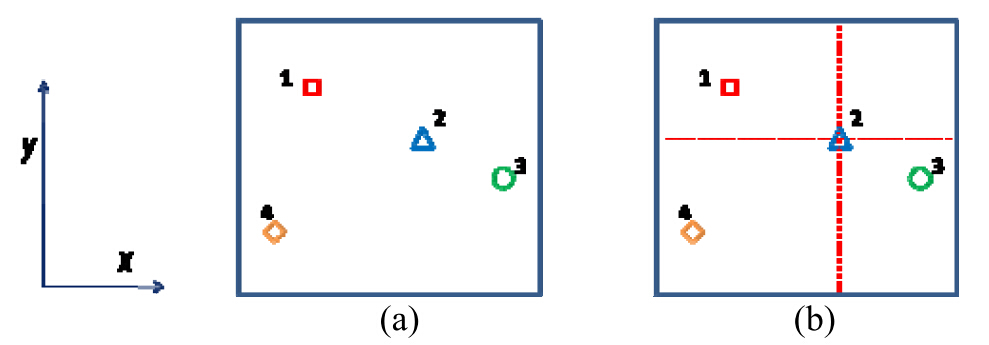
\includegraphics[width=\textwidth]{spatial_coding.jpg}
	\caption{计算$X$-map和$Y$-map示意图}\label{fig:sc}
\end{figure}
SC编码图片中每对特征点之间的相对位置关系。为了编码这种关系,SC会为每张图片生成两个空间图,称为$X$-map和$Y$-map。$X$-map编码了竖直方向上的点的相对位置关系,而$Y$-map编码了水平方向上点的相对位置关系。假设一张图片$I$有$K$个特征点$\{v_i\}$,则$I$的$X$-map和$Y$-map都是$K \times K$大小的二进制矩阵,其定义为:
\begin{equation}
X_{map}(i,j)=
\begin{cases}
0 & \text{if $x_i < x_j$} \\
1 & \text{otherwise}
\end{cases}
\end{equation}
\begin{equation}
Y_{map}(i,j)=
\begin{cases}
0 & \text{if $y_i < y_j$} \\
1 & \text{otherwise}
\end{cases}
\end{equation}
其中$(x_i,y_i)$和$(x_j,y_j)$是$v_i$和$v_j$的坐标(在图片的直角坐标系中)。图\ref{fig:sc}为计算$X$-map和$Y$-map的示意图,根据图中的例子得到的$X$-map和$Y$-map分别为:
\begin{equation}
X_{map}=
\left(
\begin{array}{cccc}
1 & 0 & 0 & 1 \\
1 & 1 & 0 & 1 \\
1 & 1 & 1 & 1 \\
0 & 0 & 0 & 1 \\
\end{array}
\right)
\end{equation}

\begin{equation}
Y_{map}=
\left(
\begin{array}{cccc}
1 & 1 & 1 & 1 \\
0 & 1 & 1 & 1 \\
0 & 0 & 1 & 1 \\
0 & 0 & 0 & 1 \\
\end{array}
\right)
\end{equation}

在得到$X$-map和$Y$-map之后就是如何使用它们进行几何校验。在检索时,对匹配的特征点进行SC校验。首先得到查询图像$I_q$和数据库图像$I_m$的SC子图$(GX_q,GY_q)$和$(GX_m,GY_m)$,然后对相应的子图进行异或操作,即:
\begin{equation}
V_x(i,j)=GX_1(i,j)\otimes GX_m(i,j)
\end{equation}
\begin{equation}
V_y(i,j)=GY_1(i,j)\otimes GY_m(i,j)
\end{equation}
异或结果中的‘1’表示不一致状态,这些不一致的总和越低两张图片的几何一致性越高,即几何一致性得分可以表示为:
\begin{equation}
S(I_q,I_m)=-\sum_{i=1}^{N}\sum_{j=1}^{N}V_x(i,j) - \sum_{i=1}^{N}\sum_{j=1}^{N}V_y(i,j)
\end{equation}


\subsubsection{Word Spatial Arrangement}
\begin{figure}[h]
	\centering
	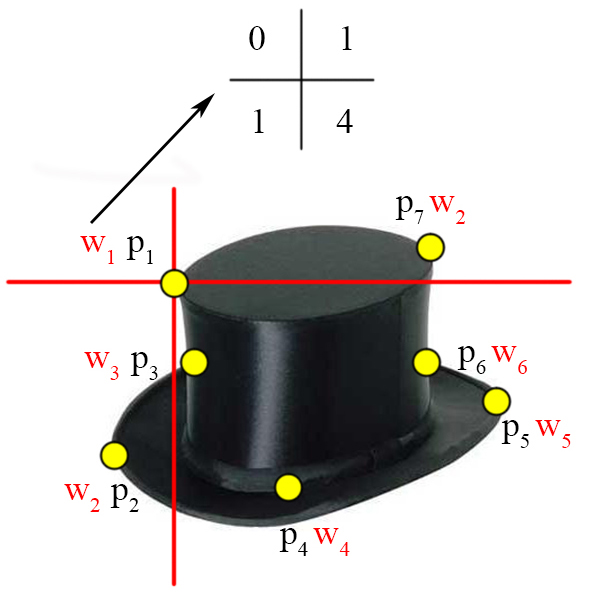
\includegraphics[width=0.5\textwidth]{WSA.jpg}
	\caption{计算WSA向量示意图}\label{fig:wsa}
\end{figure}
WSA提出了一种将特征点的相对位置关系编码到BoW向量中的算法,并在检索时校验特征点之间的几何一致性,所以WSA是一种检索时校验算法。图\ref{fig:wsa}为计算点$p_1$的WSA向量的示意图。计算WSA向量的具体算法如下:
\begin{enumerate}
	\item 将某个特征点(例如$p_1$)作为原点,建立直角坐标系,将图片分成四个象限;
	\item 统计四个象限内特征点的数目;
	\item 将这四个值进行L1归一化作为原点特征点的WSA向量;
	\item 重复上述步骤,求出图片中所有特征点的WSA向量。
\end{enumerate}

在进行检索时,对于具有相同视觉单词的点对,将他们对应WSA向量的直方图相交的值作为几何校验结果。WSA算法具有以下优点:
\begin{enumerate}
	\item 将特征点的几何关系编码到BoW向量中,在检索时进行几何校验,无需后处理,校验速度快;
	\item WSA编码特征点之间的相对位置关系,鲁棒性好;
	\item WSA可以与软量化\cite{philbin2008lost}算法结合使用。
\end{enumerate}

\subsection{现有方法的不足}
\begin{figure}[h]
	\centering
	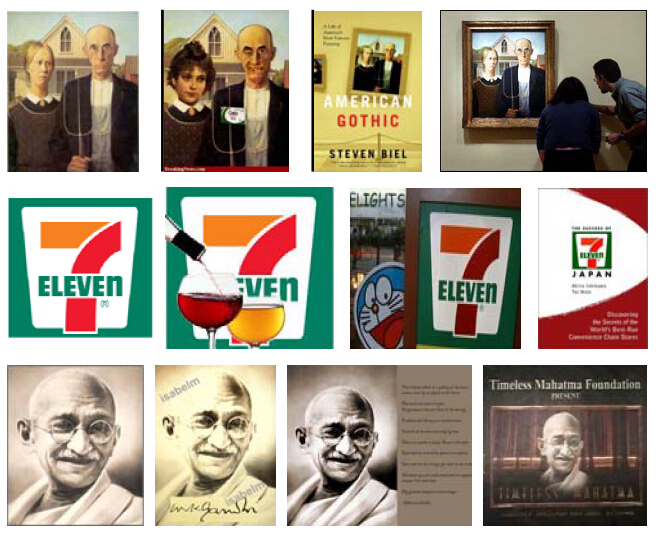
\includegraphics[width=0.7\textwidth]{sc_exa.jpg}
	\caption{部分重复(partially duplicated)相似图片}\label{fig:sce}
\end{figure}
\begin{figure}[h]
	\centering
	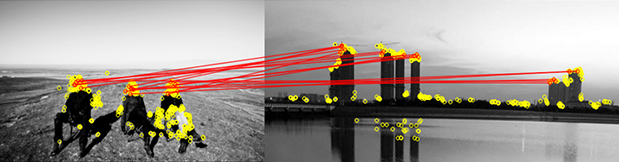
\includegraphics[width=0.8\textwidth]{WSA_exa.jpg}
	\caption{使用WSA算法后非相似图片之间特征点的匹配情况}\label{fig:wsae}
\end{figure}
以上方法虽然在某些情况下可以达到较好的校验算法,但依然存在一些问题:
\begin{enumerate}
	\item  SC几何校验算法通过二进制图编码了特征点之间严格的次序关系,这种校验算法要求图片之间有很强的相似性,甚至是在图片之间有完全一致的区域(如图\ref{fig:sce})才有比较好的效果。SC无法很好的应对更加一般的相似图像检索情况,尤其是视角、平移变化将导致二进制图较大的变化;
	\item WSA算法编码了特征点之间的相对位置关系。相比于SC,WSA算法更加鲁棒,适用于一般的检索问题。但是,图像中特征点的位置关系区分性低,无法进行较严格的几何关系校验。图\ref{fig:wsae}表明了即使考虑特征点之间的相对位置关系,还是会导致非相似图片之间的无匹配。
\end{enumerate}

本文提出的RSA算法试图解决上述问题,在完成较为严格的几何校验的同时达到一定的鲁棒性。除此之外,RSA还具有低内存消耗,低计算复杂度的特点,适用于大规模相似图像检索场景。

\section{Region Property Space}
在相似图像检索过程中提取特征的阶段,一块邻接的像素用来表述一个特征区域\cite{tuytelaars2008local},而这块区域通常用角度(angle)和尺度(scale)来描述。scale描述了这块区域覆盖的范围,而angle描述了这块区域的主方向(一般为梯度方向)。RSA将这两种属性编码到BoW向量中,并在检索时进行几何校验。因此,RSA算法需要解决两个问题:
\begin{enumerate}
	\item 如何编码视觉单词的属性信息(即angle和scale);
	\item 如何度量特征区域之间的相似性,并度量图像之间的相似性。
\end{enumerate}
第一个问题将通过本节提出的Region Property Space(RPS)来解决,而第二个问题将在Spatial Weighting章节解决。为了简化描述,在后续章节中除非明确指出,我们将不对特征点和特征区域进行区分。

\subsection{RPS的形式化定义}
\begin{figure}[h]
	\centering
	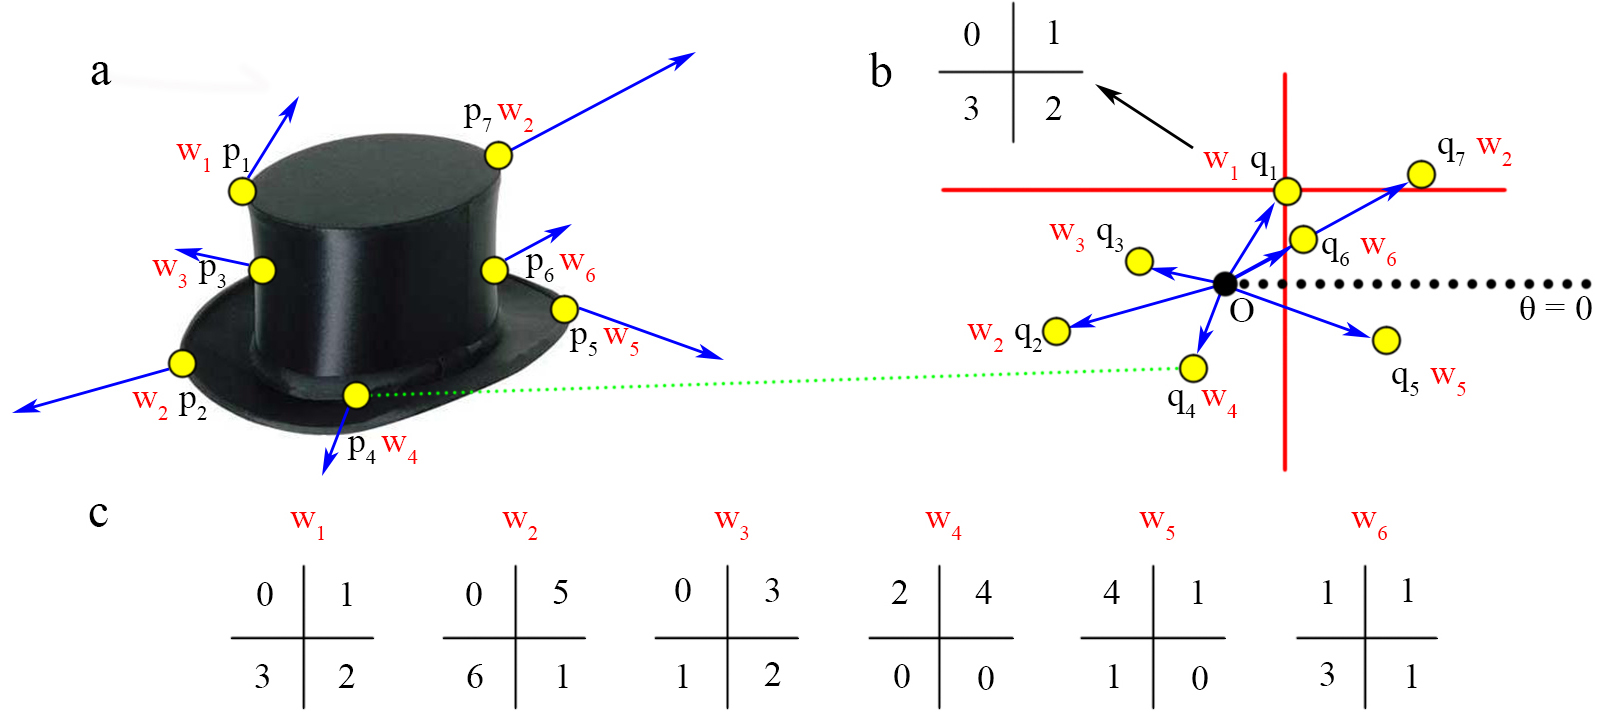
\includegraphics[width=\textwidth]{RSA.jpg}
	\caption{构建RPS和计算RSA向量实例}\label{fig:RSA}
\end{figure}
在一副图像$I$中,特征区域的集合可以表示为$R_I=\{r_I^{(1)},...,r_I^{(n)}\}$,其中$r_I^{(k)}$为第$k$个特征区域,$n$为特征区域的个数。如果只考虑特征区域的位置信息,例如\cite{lazebnik2006beyond}\cite{Cao2010Spatial}\cite{penatti2014visual}中的算法,则$R_I$将被简化为在图像直角坐标系$D$内的一个点集:
\begin{equation}
P_I=\{p_I^{(1)},...,p_I^{(n)}\}, ~~p_I^{(k)}=(x_I^{(k)},x_I^{(k)})
\end{equation}
其中,$x_I^{(k)}$和$x_I^{(k)}$表示特征区域$r_I^{(k)}$的横纵坐标。我们将这个空间定义为Region Position Space,表示为$S_{position}$。与编码$S_{position}$的信息相反,RSA试图编码特征区域的属性,即angle和scale。对于每个特征区域$r_I^{(k)} \in R_I$,它的scale和angle可以认为是在极坐标系$G$中的极径和极角,该极坐标系的极点为$O : \rho = 0$,极轴为$L : \theta = 0$。通过这种简化,我们将特征区域集合$R_I$转化为一个新的点集:
\begin{equation}
Q_I=\{q_I^{(1)},...,q_I^{(n)}\}, ~~q_I^{(k)}=(\rho_I^{(k)},\theta_I^{(k)})
\end{equation}
其中,$\rho_I^{(k)}$和$\theta_I^{(k)}$表示特征区域$r_I^{(k)}$的angle和scale。我们将这个空间定义为Region Property Space,表示为$S_{Property}$。

图\ref{fig:RSA}展示了创建$S_{Property}$的过程,其中(a)为$S_{position}$,(b)为$S_{Property}$,(c)为没有进行L1归一化的RSA向量,蓝色箭头标注了角度和尺度信息。$S_{position}$中的点与$S_{Property}$中的点具有一一对应关系,图\ref{fig:RSA}中的$p_4$和$q_4$描述了这种对应关系。通过建立$S_{Property}$,特征区域的属性的分布相当于$S_{Property}$中点的分布,并且通过这种变换,我们可以更加直接的编码属性的分布信息。图\ref{fig:RSA_dis}展示了一副典型自然图片的$S_{Property}$中的点的分布情况。
\begin{figure}[h]
	\centering
	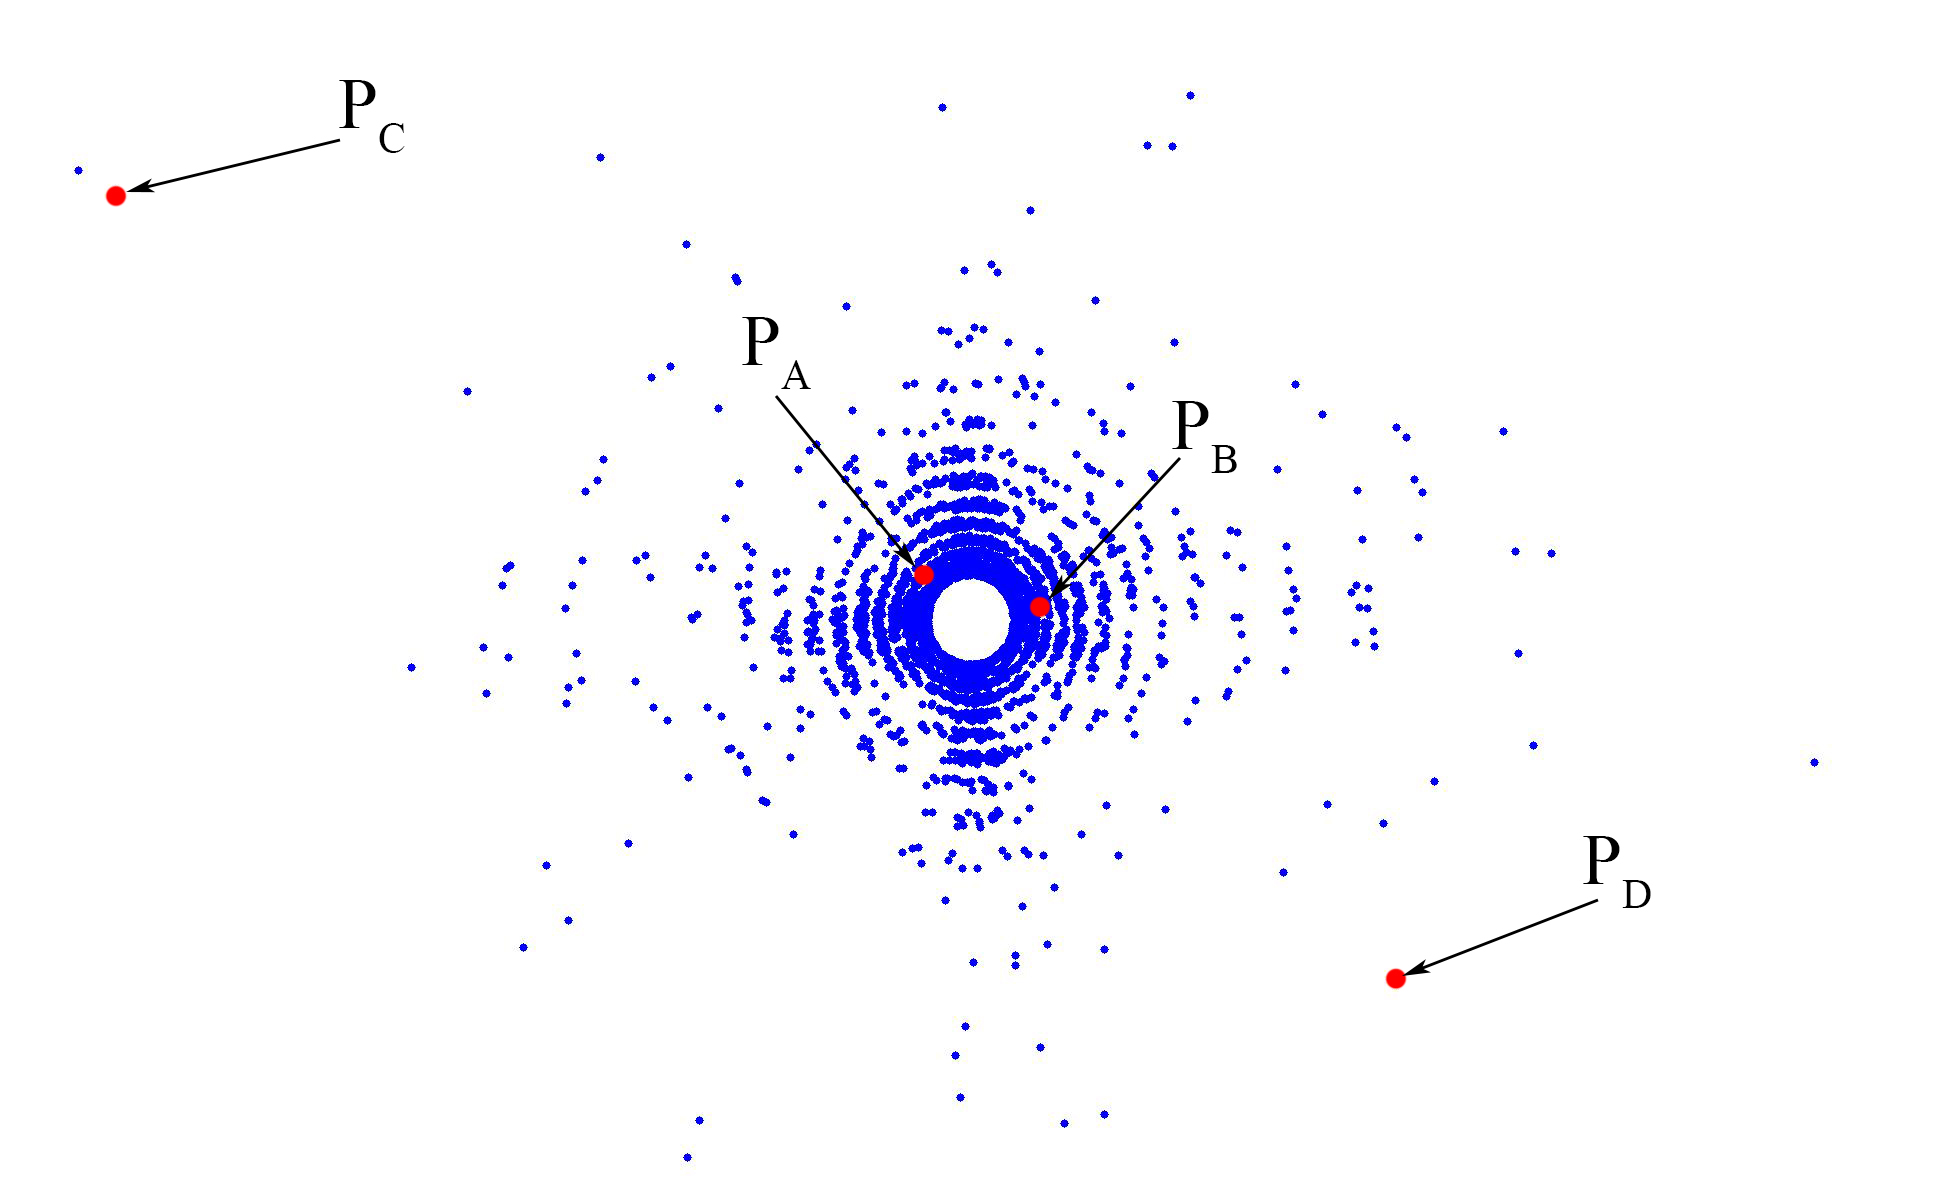
\includegraphics[width=\textwidth]{RSA_distribution.jpg}
	\caption{一幅典型自然图片的$S_{Property}$中的点的分布情况}\label{fig:RSA_dis}
\end{figure}

\subsection{RPS中点的分布}
\begin{figure}[h]
	\centering
	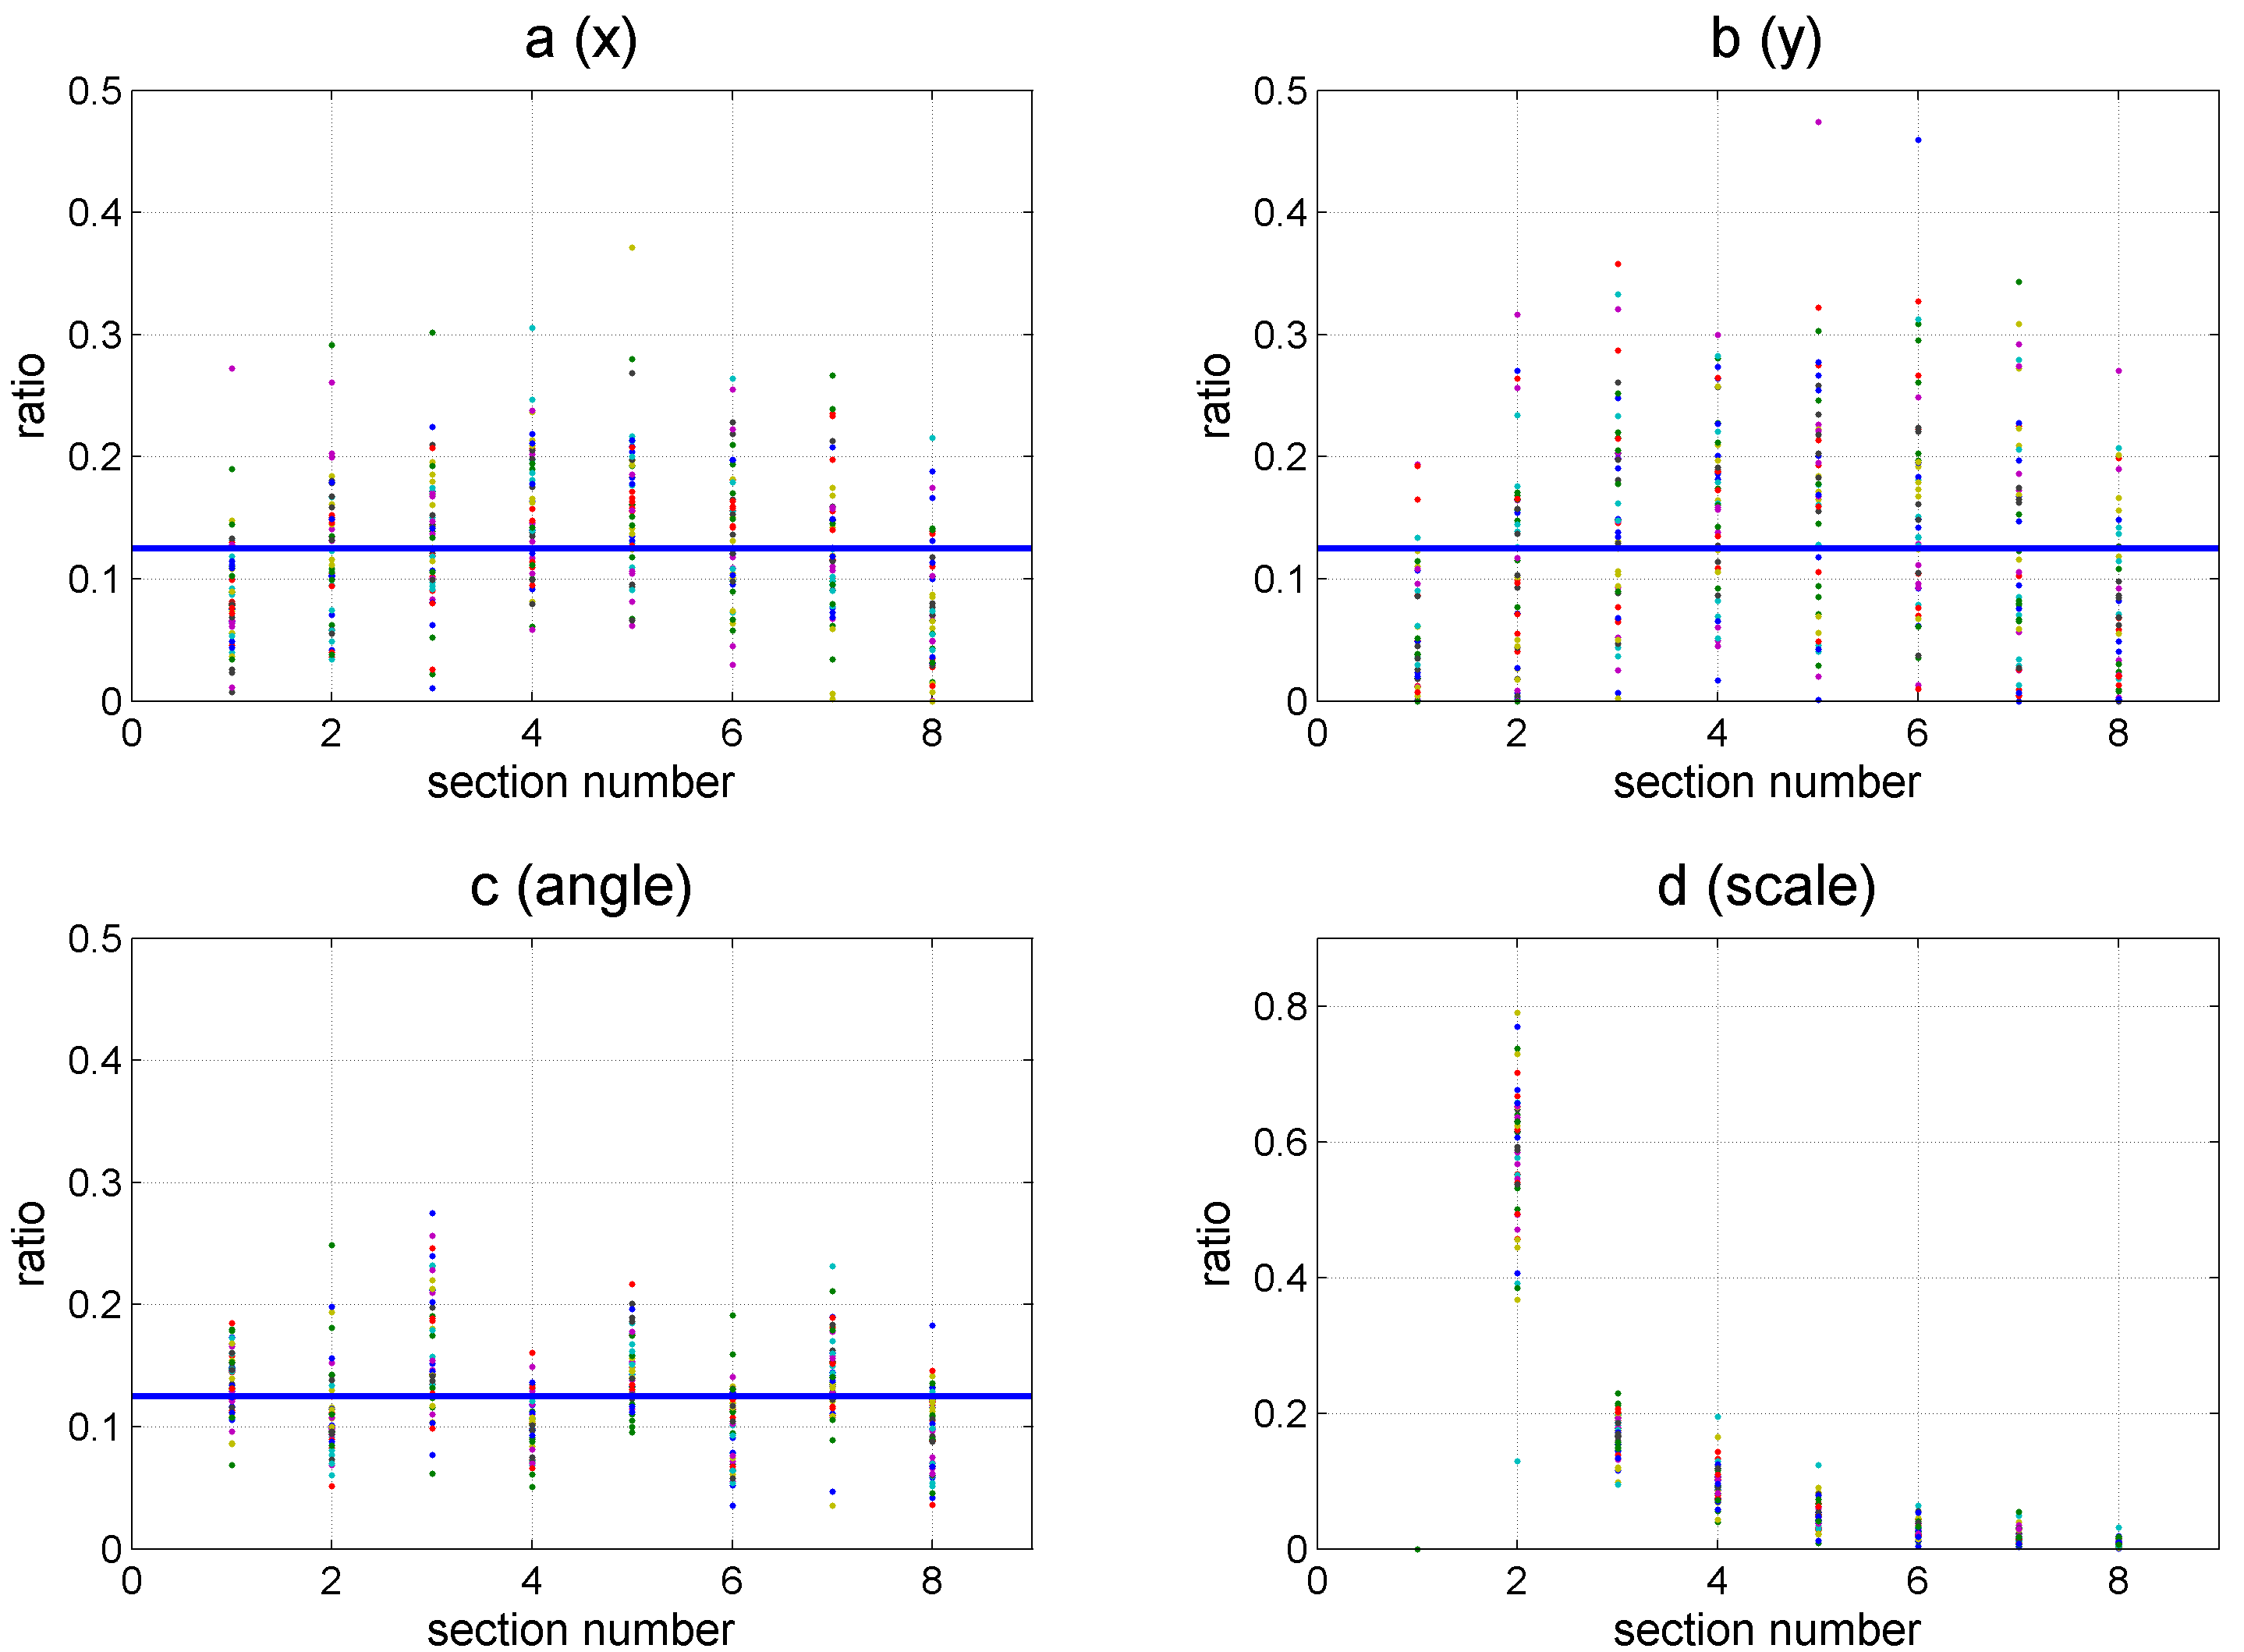
\includegraphics[width=\textwidth]{RSA_distribution_2.png}
	\caption{$S_{position}$和$S_{Property}$中的点的分布情况对比}\label{fig:RSA_dis_2}
\end{figure}
虽然在$S_{Property}$和$S_{position}$中的点存在一一映射的关系,但是他们的分布却十分不同。图\ref{fig:RSA_dis_2}展示了从Oxford\cite{philbin2007object}数据库中随机抽取的50张图片共140,000特征区域在不同空间上的分布情况。我们分别按横纵坐标将$S_{position}$分成8个区域,并统计每个区域中点的个数,如图\ref{fig:RSA_dis_2}中的(a),(b)所示。我们同样将和$S_{Property}$划分成8个区域,划分方法为:都以极点为中心,将$S_{Property}$分成8个等面积的扇形(用来测试angle的分布,如图(c))和8个等面积的同心环(用来测试scale的分布,如图(d))。图\ref{fig:RSA_dis_2}(a)、(b)、(c)中的横线为均值。通过图\ref{fig:RSA_dis_2}可以看出,在$S_{position}$中点的分布接近随机,有较大的方差,而在$S_{Property}$中angle的分布却更接近于均匀分布。在$S_{Property}$中特征区域尺度的分布更加具有规律性,我们用一个二次函数用来进行模拟:
\begin{equation}\label{eq:scale}
n=
\begin{cases}
0 & \text{$0 \le s \le s_0$} \\
\frac{1}{\alpha s^2} & \text{$s \ge s_0$}
\end{cases}
\end{equation}
其中$n$表示特征区域的个数,$s$表示特征区域的尺度值,$s_0$是cut-off尺度值,表示几乎没有特征区域的尺度会小于$s_0$,$\alpha$是一个常数。这两种截然不同的分布特性由SIFT\cite{lowe2004distinctive}描述符的提取过程确定。SIFT通过DOG\cite{lowe2004distinctive}提取图标中的blob特征,一张图片中的blob完全依赖于图片的内容。因为自然图片中的内容是随机的,所以$S_{position}$中点的分布也是随机的。但是,自然图像更加趋向于包含小的blob(一大块像素相近的区域在自然图片中并不常见,即使是像天空这样的图像,这样的区域也只有少数几个。),并且这些blob的梯度方向在360度上是均匀分布的,这就导致了图\ref{fig:RSA_dis_2}中的特殊分布规律。对于一个分布具有很强规律的点集,我们可以用相同的结构包含更多的信息。并且,我们在$S_{Property}$点的分布规律基础之上提出了计算RSA向量的快速算法和Spatial Weighting,前者提高了检索速度,后者显著提高了检索的准确度。

\section{RSA向量}
构建RSA向量的方法与构建WSA\cite{penatti2014visual}向量的算法相似,其过程如下:
\begin{enumerate}
	\item 取$S_{Property}$中的某点作为原点,将$S_{Property}$分成四个象限(水平垂直分割);
	\item 统计四个象限内特征点的数目;
	\item 将这四个值进行L1归一化作为原点特征区域的RSA向量;
	\item 重复上述步骤,求出图片中所有特征点的RSA向量。
\end{enumerate}

通过上述步骤,对于每个特征区域我们会得到一个4维的L1归一化的RSA向量。如果特征区域量化为视觉单词,那么对应的每个视觉单词就伴随一个4维的RSA向量。假设字典长度为$v$,传统BoW检索框架会对每张图片生成一个$v$维的BoW向量。当使用RSA向量时,对于每张图片我们会构建一个$4 \times v$的RSA-BoW向量。RSA-BoW向量编码了视觉单词的尺度和角度的分布信息。图\ref{fig:RSA}(b)描述了构建RSA向量的过程。需要注意的是,当两个特征区域被量化到同一个视觉单词$w_j$时(例如图\ref{fig:RSA}中的$q_2$和$q_7$),我们将他们的RSA向量相加然后进行L1归一化作为$w_j$的RSA向量,这样我们就完全抛弃了传统BoW检索框架中的词频信息。例如,在量化之前,$w_1$的RSA向量为[1, 0, 3, 2],$w_2$的RSA向量为[5, 0, 6, 1]。 同一个视觉单词的RSA向量与WSA向量\cite{penatti2014visual}没有任何数值上的关系。

\subsection{旋转的RSA向量}
只需要对上述构建RSA向量的操作稍作改进就可以使RSA达到旋转不变性。在得到RSA向量之后,我们根据特征区域的主方向(angle)重新排列RSA向量中的四个值。具体来讲,我们将RSA向量的第一维固定为这个特征区域主方向所在象限的值,其余三个值逆时针进行旋转。如\ref{fig:RSA}中的$w_2$,其主方向在第三象限,则$w_2$旋转的RSA向量为[6, 1, 5, 0]。

\section{RSA的高区分性}
\begin{figure}[h]
	\centering
	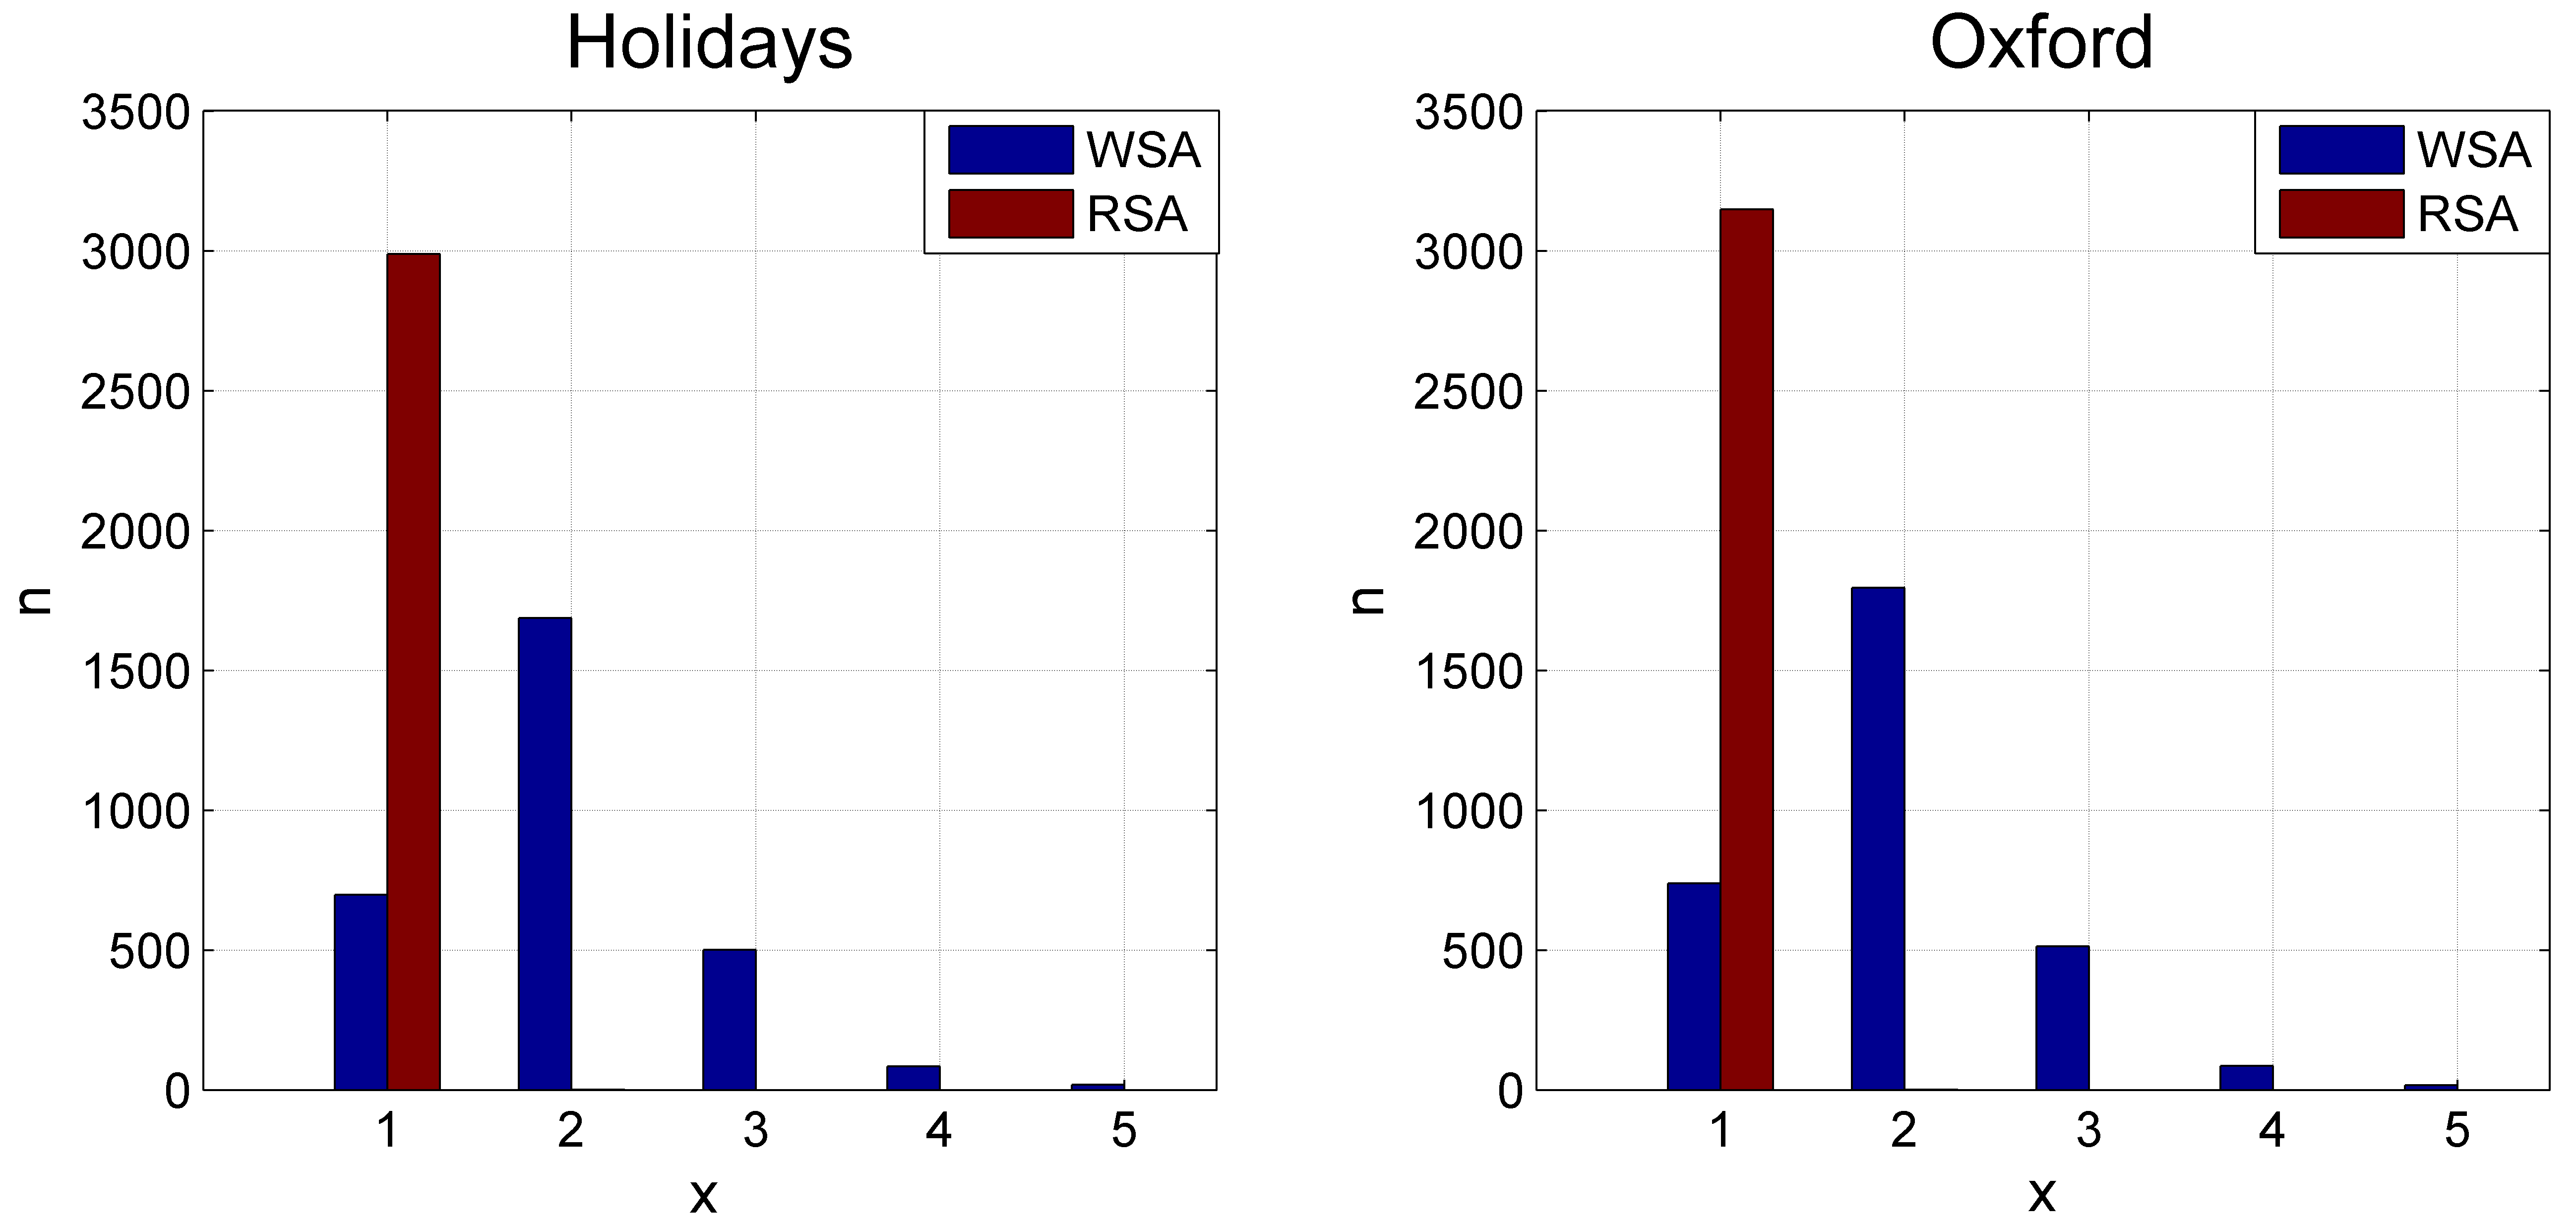
\includegraphics[width=\textwidth]{RSA_discrimination.png}
	\caption{WSA向量和RSA向量区分能力对比}\label{fig:RSA_disc}
\end{figure}
由于WSA\cite{penatti2014visual}基于特征点在图片中位置信息,所以WSA向量的值完全依赖视觉单词的坐标。但是,在实际图像检索过程中,很多特征区域的坐标是相同的。这是由于在构建SIFT\cite{lowe2004distinctive}特征时,有时候一个特征区域有不止一个主方向。此时,在同一个区域上会生成多个SIFT描述符,而它们的坐标都是一样的。这就导致了WSA向量区分能力不高,无法进行较严格的几何校验。于此相反,即使空间坐标相同,它们的梯度方向一定是不一样的,而RSA就是关注特征区域的angle和scale属性,这保证了RSA具有更高的区分能力。\ref{fig:RSA_disc}描述了WSA向量和RSA向量区分能力的对比情况。图中统计了在Holidays\cite{jegou2008hamming}数据集合Oxford\cite{philbin2007object}数据集上WSA和RSA向量的分布情况。图中的直方图(蓝色代表WSA向量,红色代表RSA向量)表示在一张图片中出现$x$次的向量平均数,例如$x=2$的cell表示在图片中出现两次的向量平均有多少。通过图\ref{fig:RSA_disc}我们可以看出,在一张图片中有75\%以上的WSA向量是重复的,而几乎没有重复的RSA向量,这证明了RSA的高区分性。

虽然在将$S_{Property}$中几乎没有重复的点,但是他们的RSA向量可以非常接近。就像在\ref{fig:RSA_dis}中的$p_A$和$p_B$。但是我们发现,这样的点几乎都分布在$S_{Property}$的原点附近,在后面章节中,我们提出了Spatial Weighting就是解决在$S_{Property}$原点附近出现的burstiness\cite{jegou2009burstiness}问题。

\section{计算RSA向量的快速算法}
为了计算一张图片所有视觉单词的RSA向量,我们需要遍历所有特征点,并且对于每个特征点,需要考虑其余特征点在$S_{Property}$的位置。这就使得计算图片RSA向量的时间复杂度为$O(n^2)$,其中$n$为图片中特征区域的个数。我们设计了一个可以更加快速计算图片所有RSA向量的算法,其核心思想很简单:
\begin{enumerate}
	\item 将$S_{Property}$按照特定的模式分成若干个区域,并统计每个区域内点的个数;
	\item 在计算某个点的RSA向量时,只对在坐标轴上的区域中的点进行重新计算。
\end{enumerate}
上述计算过程中,第一步只需要O(n)的时间复杂度,而第二步可以大大减少重复计算。

在$S_{Property}$中点规律的分布是上述思想可以对所有数据库图片有效的前提。Algorithm \ref{alg:1}给出了该算法具体的流程。
\renewcommand{\algorithmicrequire}{\textbf{Input:}} 
\renewcommand{\algorithmicensure}{\textbf{Output:}}
\begin{algorithm}
	\caption{computing the RSA vectors of an image}
	\label{alg:1} 
	\begin{algorithmic}[1]
		\REQUIRE Points set in $S_{property}$, that is $Q_I=\{q_I^{(1)},...,q_I^{(n)}\}$.
		\ENSURE RSA vectors of these points $R_I$.
		\STATE Initialize $N List$, each $List$ correspondences to a region in $S_{property}$;
		\STATE $R_I = \{\}$
		\FORALL {$q_I^{(k)}$ in $Q_I$}
		\STATE $index=$ the region that $q_I^{(k)}$ belongs to.
		\STATE put $q_I^{(k)}$ into $List[index]$.
		\ENDFOR
		\FORALL {$q_I^{(k)}$ in $Q_I$}
		\FOR {$i=0$ to $N-1$}
		\IF {$List[i]$ on the axes}
		\STATE re-count the points in $List[i]$.
		\ENDIF
		\ENDFOR
		\STATE update $R_I[k]$
		\ENDFOR
	\end{algorithmic} 
\end{algorithm}

我们设计了三种模式来划分$S_{Property}$,如图\ref{fig:RSA_d}。这三种模式分布将分$S_{Property}$分成了8、16和25个区域,并且在划分时我们考虑了点在$S_{Property}$中的分布特性,尽量使每个区域中点的数目均衡。算上暴力算法(可以认为只将$S_{Property}$划分成一个区域的特殊情况),我们将这四种算法的结果列在表\ref{tab:divide}中。我们列出了计算Holidays数据集所有图片的RSA向量所需的时间和对应的理论加速比(theoretical SR)和实际加速比(actual SR),theoretical  SR和actual SR的定义如下:
\begin{equation}
theoretical-SR = \frac{\#\text{all regions}}{\#\text{regions on axes}}
\end{equation}
\begin{equation}
actual-SR = \frac{time(\text{brute\_force})}{time(\text{divide\_x})}
\end{equation}
其中$\#$表示计数,$time()$表示所需时间。通过表\ref{tab:divide}我们可以看出,如果$S_{Property}$的分割模式与$S_{Property}$中点的分布契合,实际的加速比将逼近于理论加速比。由于在$S_{position}$中点的分布不具有$S_{Property}$中的规律性,无法得到最优的划分模式,所以这里提出的加速算法只适用于RSA向量的计算。

\begin{figure}[h]
	\centering
	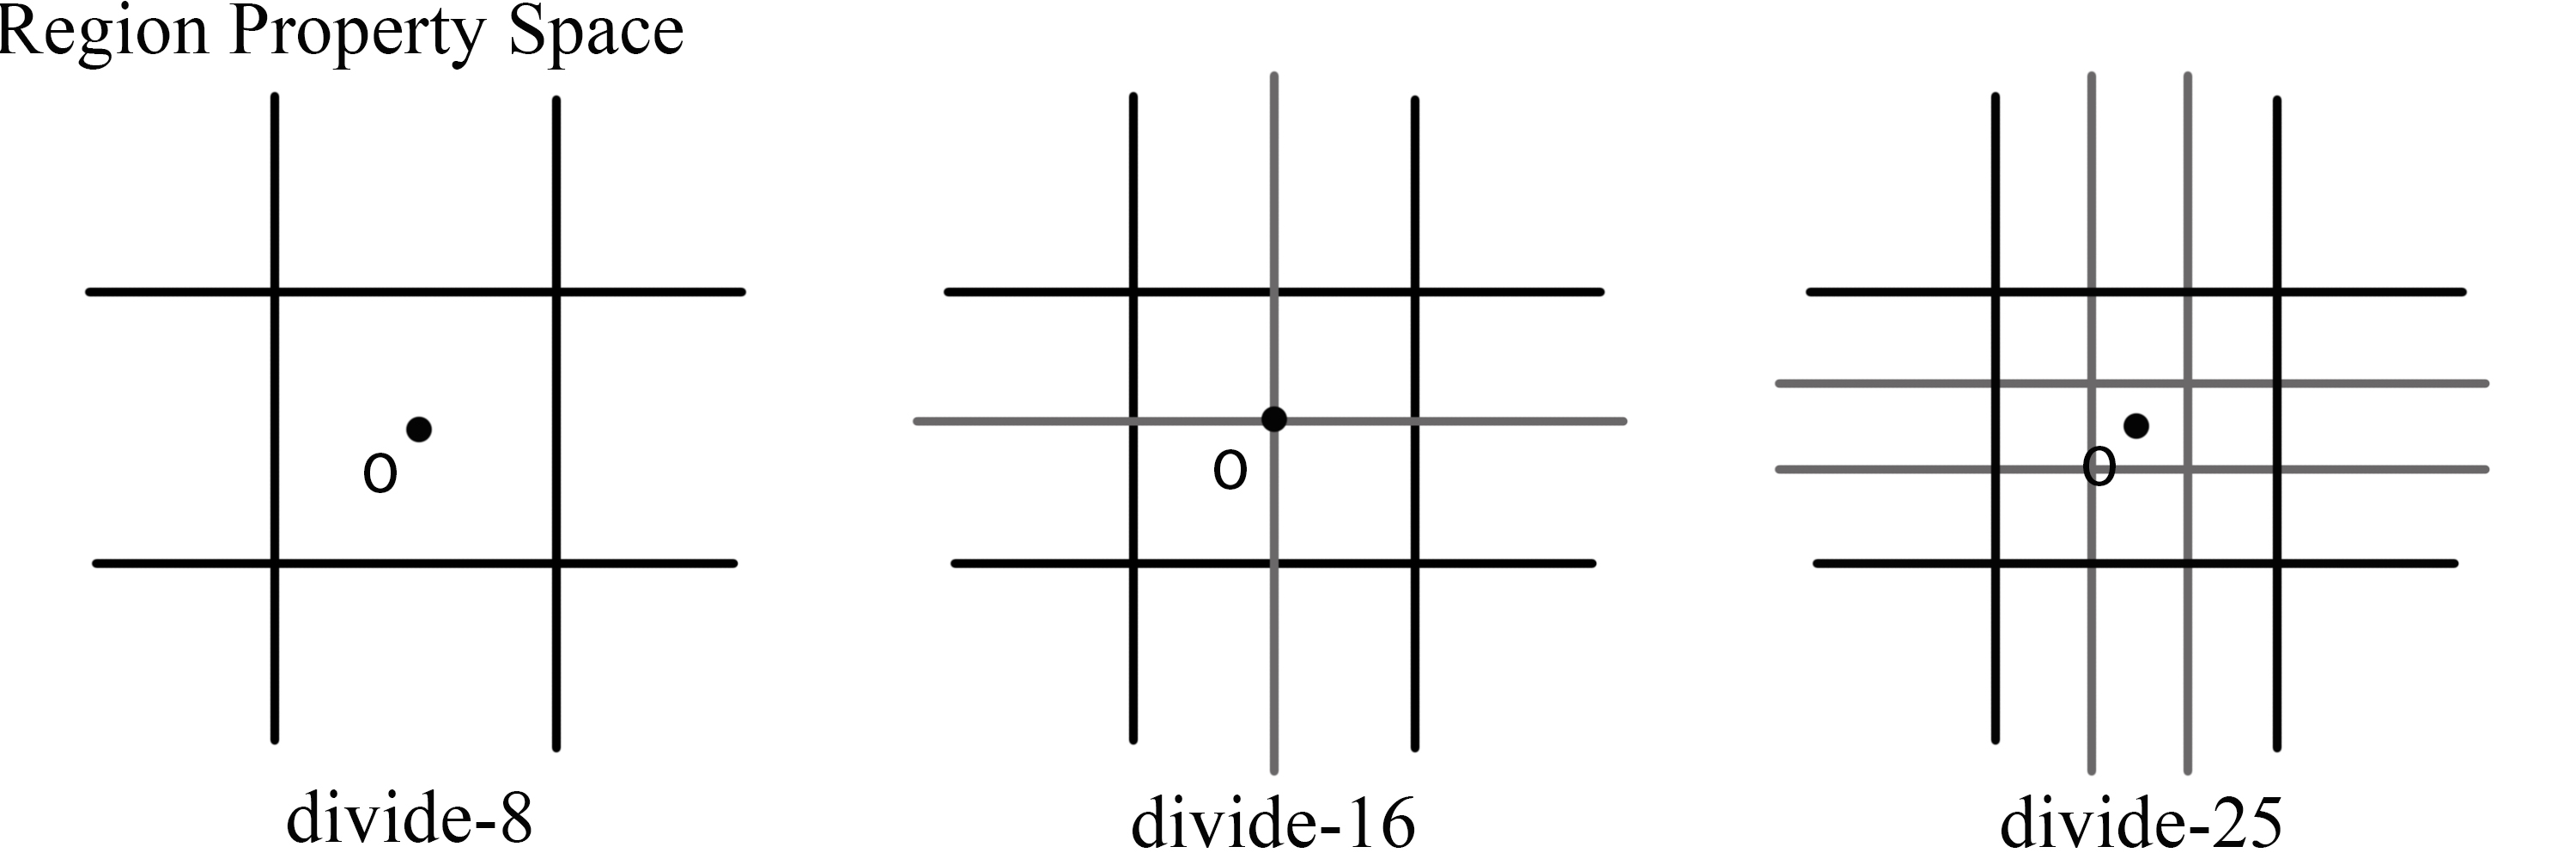
\includegraphics[width=\textwidth]{RSA_divide.jpg}
	\caption{划分$S_{Property}$的三种模式}\label{fig:RSA_d}
\end{figure}

\begin{table}
	\begin{center}
		\begin{tabular}{|l|c|c|c|c|}
			\hline
			& brute-force & divide-8  & divide-16 & divide-25 \\
			\hline
			time(s)    		& 461.4       & 281.8     & 200.7     & 187.7 \\
			theoretical SR	& 1.00        & 1.80      & 2.29      & 2.8 \\
			actual SR		& 1.00        & 1.64      & 2.28      & 2.45 \\    
			\hline
		\end{tabular}
	\end{center}
	\caption{使用不同算法计算RSA向量的时间复杂度对比}
	\label{tab:divide}
\end{table}

\section{Spatial Weighting}
\subsection{相似度计算}
在使用RSA进行图像检索时,通过公式\ref{eq:sim1}来计算图像之间的相似度。
\begin{equation}\label{eq:sim1}
S_{QI} = \frac{\sum_{j=1}^vsum(RSA_j^Q \cap RSA_j^I)}{N_Q + N_I}
\end{equation}

其中,$S_{QI}$表示查询图片$Q$和数据库图片$I$之间的相似性,$v$是视觉字典的长度;$(RSA_j^Q \cap RSA_j^I)$表示$Q$和$I$的第$i$个RSA向量的直方图相交的结果;$sum$表示向量中每一维的总和;$N_Q$和$N_I$表示图片$Q$和$I$包含的特征数。

\subsection{Burstiness}
\begin{figure}[h]
	\centering
	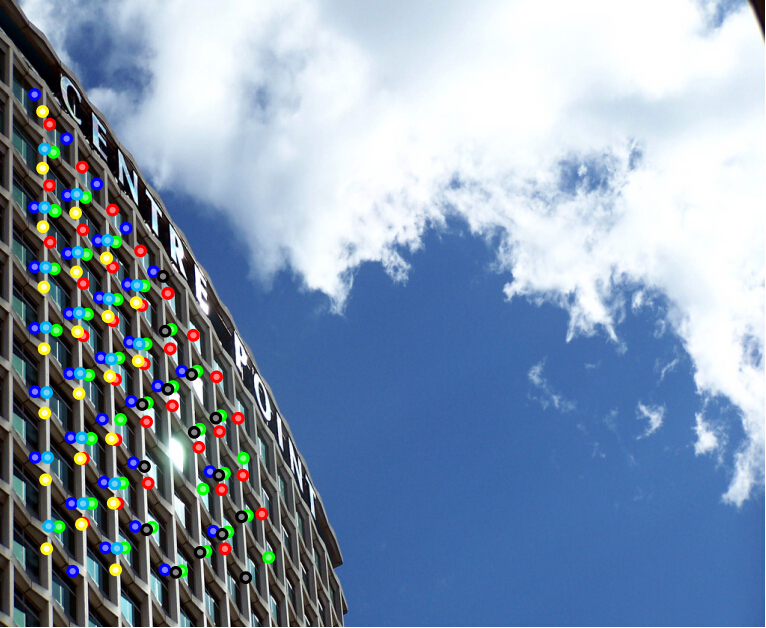
\includegraphics[width=0.8\textwidth]{burstiness.jpg}
	\caption{图像检索中的burstiness现象}\label{fig:burst}
\end{figure}

由于图片中大量存在重复的结构,如自然图片中的草地的纹理、建筑物图片中的窗户等,因此burstiness\cite{jegou2009burstiness}在图片检索中是一种常见的现象。burstiness现象最初发现于文本检索中。人们发现当某篇文档中出现了某个特定的单词,那么这个单词极有可能在该文档中还会出现。在基于BoW的图像检索框架中同样存在burstiness现象,图\ref{fig:burst}就描绘除了一张建筑物图片中存在的burstiness现象。burstiness现象会严重影响图像检索的精度,因为它过分增加了某些特征的重要性。在传统的TF-IDF加权模型中,由于burstiness现象,某些视觉单词的TF值会非常大,导致检索时的误匹配。例如,在检索过程中,如果一张数据库图片包含了图\ref{fig:burst}中的burstiness视觉单词,则该视觉单词会与所有图\ref{fig:burst}中的这些视觉单词匹配,导致严重的误匹配。

人们对图像检索中的burstiness现象同样进行了广泛的研究:\cite{Zhong2015Fast}提出了使用$1+\log (tf)$替换TF-IDF中的$tf$项来降低词频过高的影响;\cite{jegou2008hamming}深入研究了intra-image和inter-image的burstiness现象,并且提出相应的解决方案,在检索时减少误匹配的发生;\cite{shi2015early}通过统计学的方法,在进行检索前发现并去除burstiness的视觉单词。

\subsection{改进的相似度计算}
在基于RSA几何校验的图像检索方案中,同样存在burstiness的问题。如图\ref{fig:RSA_dis}中所示,接近$S_{Property}$极点的视觉单词将具有相似的RSA向量,这同样会导致在检索时产生误匹配。基于$S_{Property}$中点特殊的分布模式,对此我们提出了一种新的加权方案Spatial Weighting(SpW)。相比于TF-IDF加权模型,SpW是一种局部的加权方案,这是由于计算SpW时,只考虑对应两个视觉单词在$S_{Property}$中的位置关系。通过公式\ref{eq:scale}我们可以看出一个特征区域更加趋向于有较小的scale,因而它在$S_{Property}$中更可能位于极点附近,我们将这种特征区域标记为$q_s$。于此相反,我们将那些具有较大尺度,远离极点的特征区域标记为$q_l$。$q_s$和$q_l$具有以下特点:
\begin{enumerate}
	\item 在一张图片中$q_s$出现的概率高,并且$q_s$所对应的RSA向量的四个值的方差较小;
	\item 在一张图片中$q_l$出现的概率低,并且$q_l$所对应的RSA向量的四个值的方差较大,一般具有一个或两个峰值;
	\item 在检索时$q_s$容易发生误匹配,而$q_l$不容易发生误匹配。
\end{enumerate}

SpW的思想就是减小$q_s$的权重,增加$q_l$的权重,所以改进的相似度计算公式如下:
\begin{equation} \label{eq:sim2}
S_{QI} = \frac{\sum_{j=1}^vspw_j \times sum(RSA_j^Q \cap RSA_j^I)}{N_Q + N_I}
\end{equation}
其中,
\begin{equation} \label{eq:sim3}
spw_j = (\max(RSA_j^Q \cap RSA_j^I))^r
\end{equation}

其中,$r$控制了SpW权重施加的力度。实验表明,当$r=2$时可以达到最优的检索精度,这也符合公式\ref{eq:scale}。SpW具有以下优点:
\begin{enumerate}
	\item 计算复杂度低,几乎不增加检索时间;
	\item 可以一定程度上减弱burstiness现象对检索性能的影响;
	\item 可以保证正确的匹配具有较大的权重。
\end{enumerate}

\section{大规模图像检索框架}
在进行大规模的图像检索,尤其是图片数据规模在百万以上时,要求检索引擎有较快的相应时间和低内存占用。为此,我们提出了量化的RSA向量,并将RSA向量直接编码到倒排表中,保证了检索的性能。

\subsection{量化的RSA向量}
如果直接的表示一个RSA向量,则我们需要4个浮点数,这是传统的BoW模型的四倍($tf\_idf$值只需要一个浮点数表示)。为了可以节省空间,我们将RSA向量进行量化,每个RSA浮点数被量化到一个无符号的字符类型(8 比特),这样表示一个RSA向量只需要32比特,相当于一个浮点数,与传统的BoW模型占用相同的内存。表\ref{tab:quantization}列出了在三个数据集上量化对RSA效果的影响,其中“Original”表示没有进行量化,“Quantized”表示进行了量化。通过表\ref{tab:quantization}我们发现,量化操作并没有明显的影响RSA的性能,这可能是由于RSA原本就是编码图片的全局信息,抗噪声能力强,量化的RSA保持了它的高区分能力。这同时也证明了RSA适合大规模检索的应用。在实验部分,所有RSA向量都是经过量化的。
\begin{table}
	\begin{center}
		\begin{tabular}{|c|c|c|c|}
			\hline
			& Holidays       & Oxford5K         & Paris\\
			& 20K~~~~~ 200K  & 500K~~~~ 1M    & 500K~~~~ 1M\\
			\hline\hline
			Original    & 0.631 ~ 0.691  & 0.754 ~ 0.803  & 0.781 ~ 0.795\\
			Quantized	& 0.627 ~ 0.690  & 0.760 ~ 0.809  & 0.772 ~ 0.796\\
			\hline
		\end{tabular}
	\end{center}
	\caption{量化与非量化的RSA性能对比} 
	\label{tab:quantization}
\end{table}

\subsection{倒排索引结构}
在进行大规模图像检索时,我们同样使用经典的倒排索引结构。图\ref{fig:ii}显示了我们的倒排索引结构:每个视觉单词指向了一个包含该视觉单词的列表;在该列表中,除了包含必须的图片ID外,还包含了该视觉单词在该图片中的RSA向量值。通过量化操作,该倒排表与传统的BoW模型中的倒排表占用相同的内存。图像检索过程相当于累加RSA向量相似度得分的过程,一张图片的最终得分为加权的RSA向量相似度得分和。
\begin{figure}[h]
	\centering
	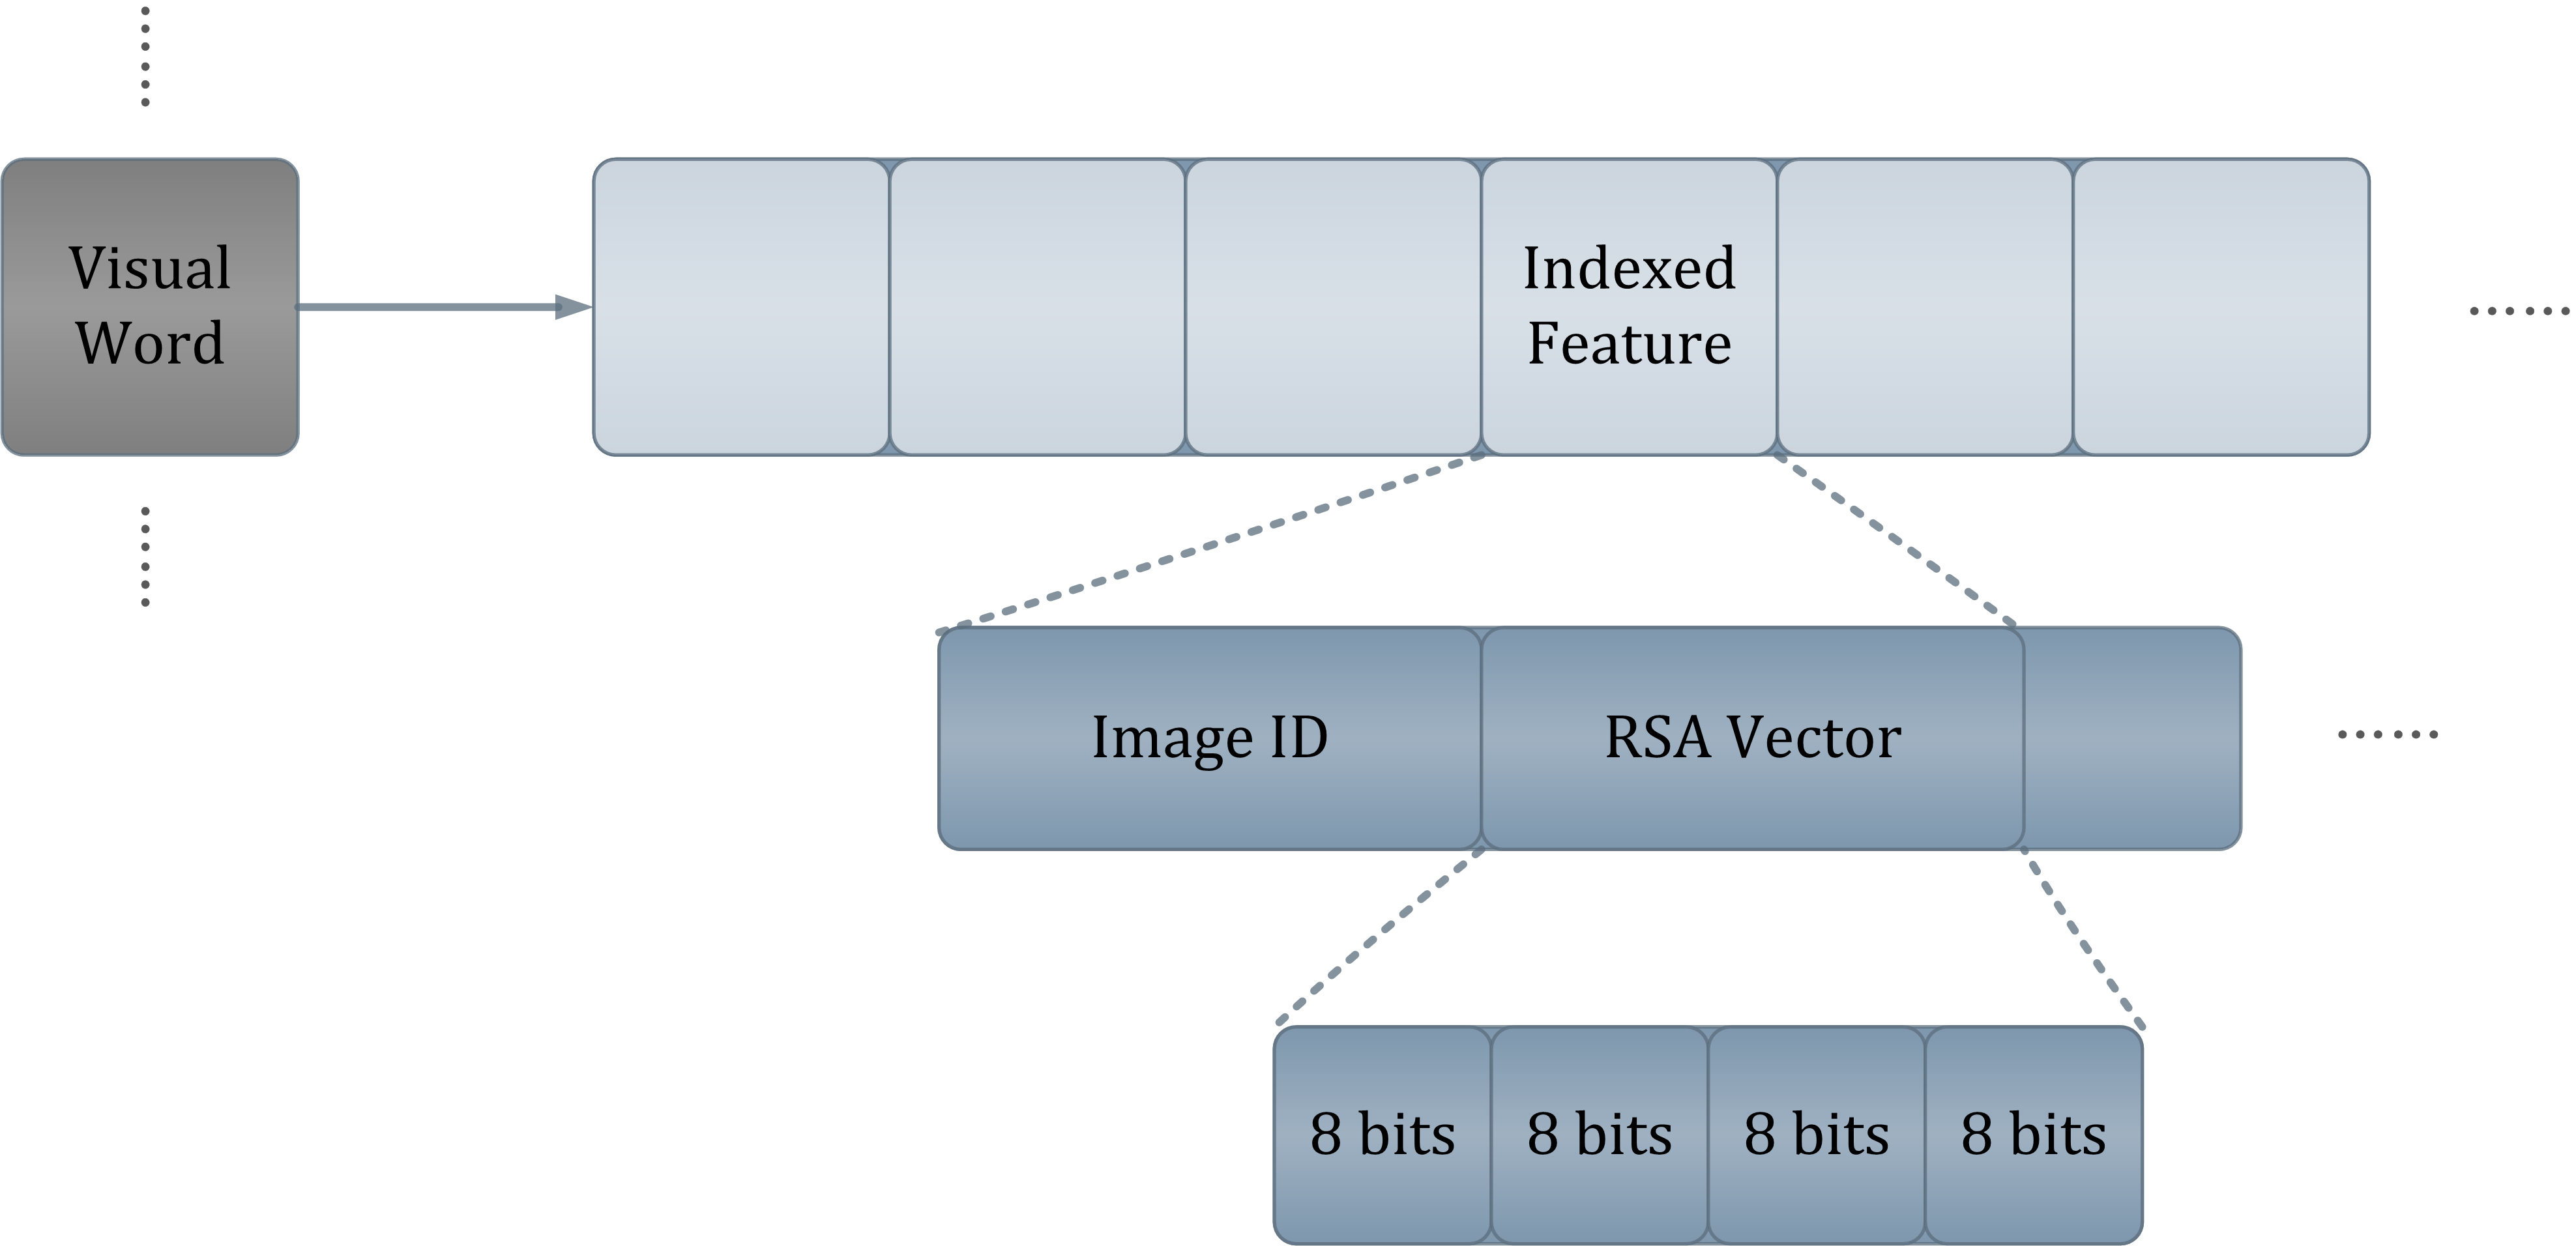
\includegraphics[width=0.8\textwidth]{Inverted_Index.png}
	\caption{包含RSA的倒排索引结构}\label{fig:ii}
\end{figure}


\section{实验}
我们的实验主要在Holidays\cite{jegou2008hamming}、Oxford5K\cite{philbin2007object}和Paris\cite{philbin2008lost}三个标准数据集上进行。这三个数据集可以测试多种变换和检索精度。在具体实验过程中,我们首先检测图片中的Hessian-Affine区域\cite{mikolajczyk2004scale},并在该区域上提取SIFT局部特征\cite{lowe2004distinctive}。为了应对实际图像检索中可能出现的旋转问题,我们并没有应用重力向量假设\cite{perd2009efficient}。为了快速构建视觉词典,我们使用了AKM\cite{philbin2007object}聚类算法。为了提高baseline,我们使用了改进的SIFT特征RootSIFT\cite{arandjelovic2012three}。为了可以与其他算法进行比较,我们使用标准的实验的参数:对于Holidays数据集,我们在一个独立的数据集上建立200K的视觉词典;对于Oxford5K和Paris我们构建了1M的视觉字典,并且考虑查询图片的输入区域。为了验证RSA算法在大规模数据库上的性能,我们测试了在Holidays+Flickr1M\cite{philbin2007object}上图像检索的性能。由于Holidays、Oxford5K和Paris无法测试尺度变换,我们在Copydays\cite{douze2009evaluation}上测试了RSA对尺度变化的鲁棒性。在Holidays数据集上,我们使用旋转的RSA向量,这是由于只有Holidays数据集中的图片可能有不同的方向。我们使用mAP(Mean Average  Pecision)度量检索的性能。

\subsection{数据集}

\subsubsection{Holidays}
Holidays数据集包含1,491张各种场景的图片。其中500张查询图片,并且大部分查询图片对应一到两张相似图片。该数据集可以测试图像检索中旋转、视角变换、模糊等情况。

\subsubsection{Oxford5K}
Oxford5K的5,062张图片包含了11个Oxford的地标性建筑。每个地标有5张查询图片,所以共有55张查询图片。每张数据库图片被分成以下等级:
\begin{enumerate}
	\item Good,相应的地标完整的显示在图片内;
	\item Ok,相应的地标至少有25\%的部分显示在图片内;
	\item Junk,无法确定其与地标的相关性;
	\item Absent,相应的地标不在图片内;
\end{enumerate}

根据一般规则,我们在计算mAP时不考虑标注为Junk的图片。

\subsubsection{Paris}
Paris数据集包含6,412张图片,这些图片通过在Flickr上搜索“paris landmarks”得到。Paris数据集同样包含55张查询图片,并且数据库图片具有与Oxford5K相似的标签。

\subsubsection{Copydays}
Copydays数据集包含了Holidays数据集中的157张图片。每张图片进行了人工处理,包括JPEG压缩、裁剪和其他变换。我们只使用经过JPEG压缩的部分数据。在这部分数据中,每张图片经过不同程度的压缩,包含9个等级,质量值范围为75至3。所以,我们共使用了1,570张图片。在这个数据集上我们使用topN检索图片的准确率(P@N)来度量检索性能。

\subsubsection{Flicker1M}
这个数据集包含从Flickr上下载的1,040,801张图片,主要用于测试算法的可扩展性。

\subsection{参数影响}
通过\ref{eq:sim2}和\ref{eq:sim3}我们可以发现,RSA的检索性能只由字典大小$v$和权重影响因子$r$来决定。这节将讨论这两个参数的影响并得到最优值。
\begin{figure}[h]
	\centering
	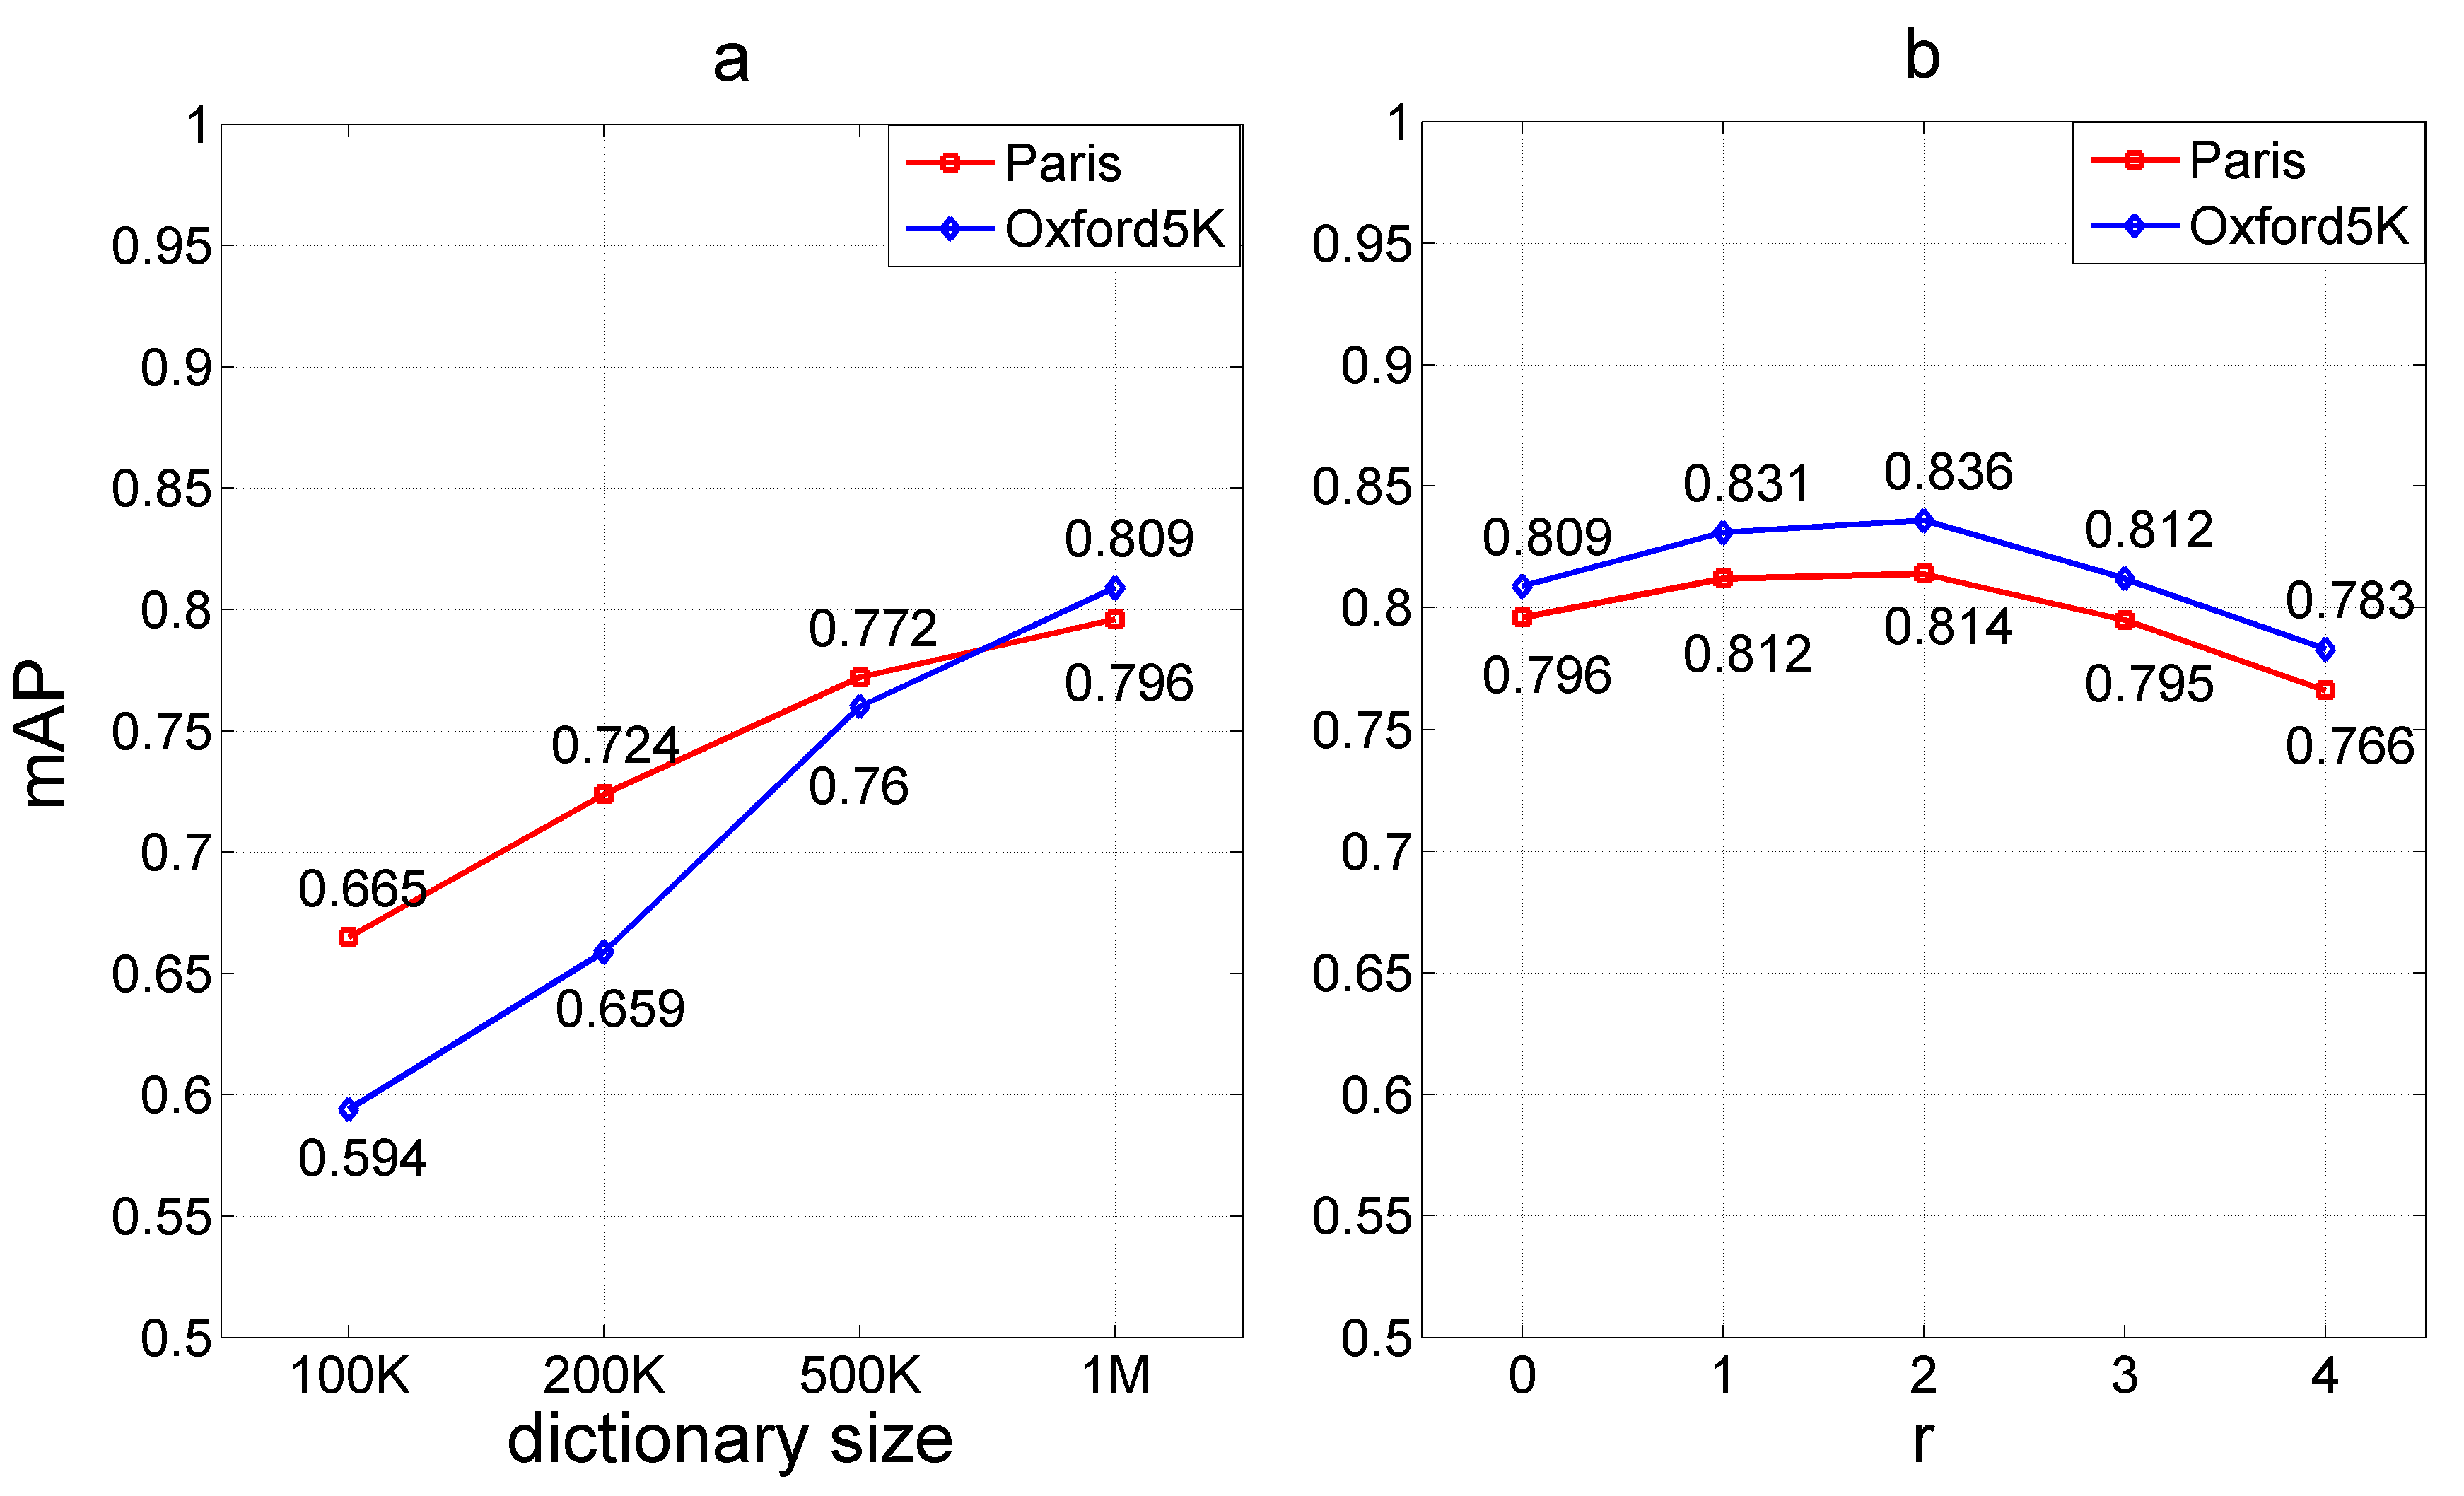
\includegraphics[width=0.8\textwidth]{dic_r.png}
	\caption{(a)字典大小对检索结果的影响;(b)权重影响因子$r$对检索效果的影响}\label{fig:dr}
\end{figure}

\subsubsection{字典大小$v$}
\ref{fig:dr}(a)给出了字典大小对检索结果的影响(没有使用SpW的情况),我们在Oxford 5K和Paris两个数据库上使用四种大小的字典进行了实验。通过实验结果可以看出,当字典变大时RSA会取得更好的检索mAP。其原因不仅是大字典可以增加视觉单词的区分能力,同时也提高的RSA向量的区分力。在计算RSA向量时,不同的特征区域可能会被量化到同一个视觉单词,这会导致其RSA的区分能力下降。较大的字典可以减少这种现象出现的概率。

\subsubsection{权重影响因子$r$}
SpW的目标是减弱在检索过中的burstiness现象,即在$S_{Property}$中,在极点附近出现点的概率要明显高于周围出现点的概率。参数$r$控制了SpW施加的力度,也就是对极点附件点权重的抑制程度,$r$越大,极点附近点的权重就越低。理论上,当$r$的取值符合公式\ref{eq:scale}中刻画的分布情况时,SpW达到最优的检索效果。图\ref{fig:dr}(b)展示了$r$不同取值下的mAP。通过该实验可以看出,当$r=2$时,SpW达到最优的性能,这也是符合我们的期望的。在后续的试验中,我们固定$r=2$。

\subsection{RSA和SpW的性能}
\begin{table}
	\begin{center}
		\begin{tabular}{|c|c|c|c|}
			\hline
			& Holidays       & Oxford5K         & Paris\\
			& 20K~~~~~ 200K  & 500K~~~~ 1M    & 500K~~~~ 1M\\
			\hline\hline
			baseline  & 0.566 ~ 0.611  & 0.651 ~ 0.685  & 0.674 ~ 0.681\\
			\hline
			~WSA      & 0.721 ~ 0.742  & 0.743 ~ 0.792  & 0.779 ~ 0.804\\
			*WSA      & 0.717 ~ 0.737  & 0.764 ~ 0.793  & 0.783 ~ 0.790\\
			\hline
			~RSA      & 0.757 ~ 0.775  & 0.760 ~ 0.809  & 0.772 ~ 0.796\\
			*RSA      & \textbf{0.800} ~ \textbf{0.806} & \textbf{0.802} ~ \textbf{0.836} & \textbf{0.803} ~ \textbf{0.814}\\
			\hline
		\end{tabular}
	\end{center}
	\caption{在Holidays、Oxford5K和Paris数据集上的检索结果}
	\label{tab:map1}
\end{table}

表\ref{tab:map1}比较了RSA与BoW baseline和WSA\cite{penatti2014visual}的检索性能,其中*表示使用SpW。为了使RSA方法达到较高的检索精度,在Holidays数据集的试验中,我们融合了HE\cite{jegou2008hamming}和HE Weighting\cite{jegou2009burstiness}方法。通过表\ref{tab:map1}可以看出,WSA和RSA对BoW baseline都有明显的提升,尤其是RSA算法。RSA算法在大多数情况下都比WSA得到更优的检索结果。因为RSA只编码了特征区域的属性信息,所以我们可以得出结论:特征区域的属性信息要比特征区域的位置信息\cite{penatti2014visual},和在图片中出现的频率信息具有更高的区分能力。

\subsubsection{SpW带来的提升}
SpW带来的效果提升是很明显的。在Holiday O型和Oxford5K数据集上,SpW可以将RSA的结果提升5\%;在Paris数据集上,SpW同样可以带来4\%的提升。SpW的设计针对$S_{Property}$点的特殊分布模式,所以SpW对WSA算法没有效果。

\subsubsection{与其他空间校验算法的比较}
\begin{table}
	\begin{center}
		\begin{tabular}{|c|c|c|c|c|c|c|}
			\hline
			Dataset   & RSA     & \cite{jegou2009burstiness}   &\cite{wang2011contextual}    & \cite{Zhong2015Fast}    & \cite{Zhong2015Fast}(gv)  &\cite{babenko2014neural}\\
			\hline\hline
			Oxford5K  & 0.836   & -      & -      & 0.746  & \textbf{0.850}  & 0.557\\
			\hline
			Paris     & \textbf{0.814}   & -      & -      & 0.725  & \textbf{0.814}  & -\\
			\hline
			Holidays  & 0.806   & \textbf{0.807}  & 0.780  & 0.720  & 0.771  & 0.789\\
			\hline
		\end{tabular}
	\end{center}
	\caption{RSA与state-of-the-art算法的比较}
	\label{tab:map2}
\end{table}

我们将RSA算法与目前比较优秀的几何校验算法进行了比较,包括WGC\cite{jegou2008hamming}\cite{jegou2009burstiness},SCW\cite{wang2011contextual},DSM\cite{Zhong2015Fast}和Neural Code\cite{babenko2014neural}。表\ref{tab:map2}列出了比较的结果,其中gv表示使用了重力向量假设。通过表\ref{tab:map2},我们发现RSA在Holidays数据集上得到了与\cite{jegou2009burstiness}相近的结果。但是由于RSA将空间信息编码到BoW向量中,在检索时完成校验,而WGC是一种后检验方法,所以RSA在检索效率上要高于WGC,这点可以通过表\ref{tab:time}得到验证。具有重力向量假设的DSM在Paris得到了与RSA相同的结果,并在Oxford5K上得到了高于RSA的结果。DSM得到的高mAP是因为它使用了更加严格的限制,但是在实际的图像检索的场景下,图片旋转是很常见的,此时无法保证重力向量假设。在同样使用普通的SIFT描述符\cite{lowe2004distinctive}时,RSA的检索结果要远远高于DSM。所以,相比于DSM,RSA更适合一般情况下的大规模图像检索。

\begin{table}
	\begin{center}
		\begin{tabular}{|c|c|c|c|c|}
			\hline
			Method         & RSA & baseline & \cite{jegou2009burstiness} & \cite{wang2011contextual}\\
			\hline
			Query Time (s) & 0.625 & 0.623 & 0.858 & 0.676\\
			\hline
		\end{tabular}
	\end{center}
	\caption{在Holidays+Flickr1M数据集上不同算法的查询时间(单核CPU)}
	\label{tab:time}
\end{table}

\subsubsection{大规模图像检索}
\begin{figure}[h]
	\centering
	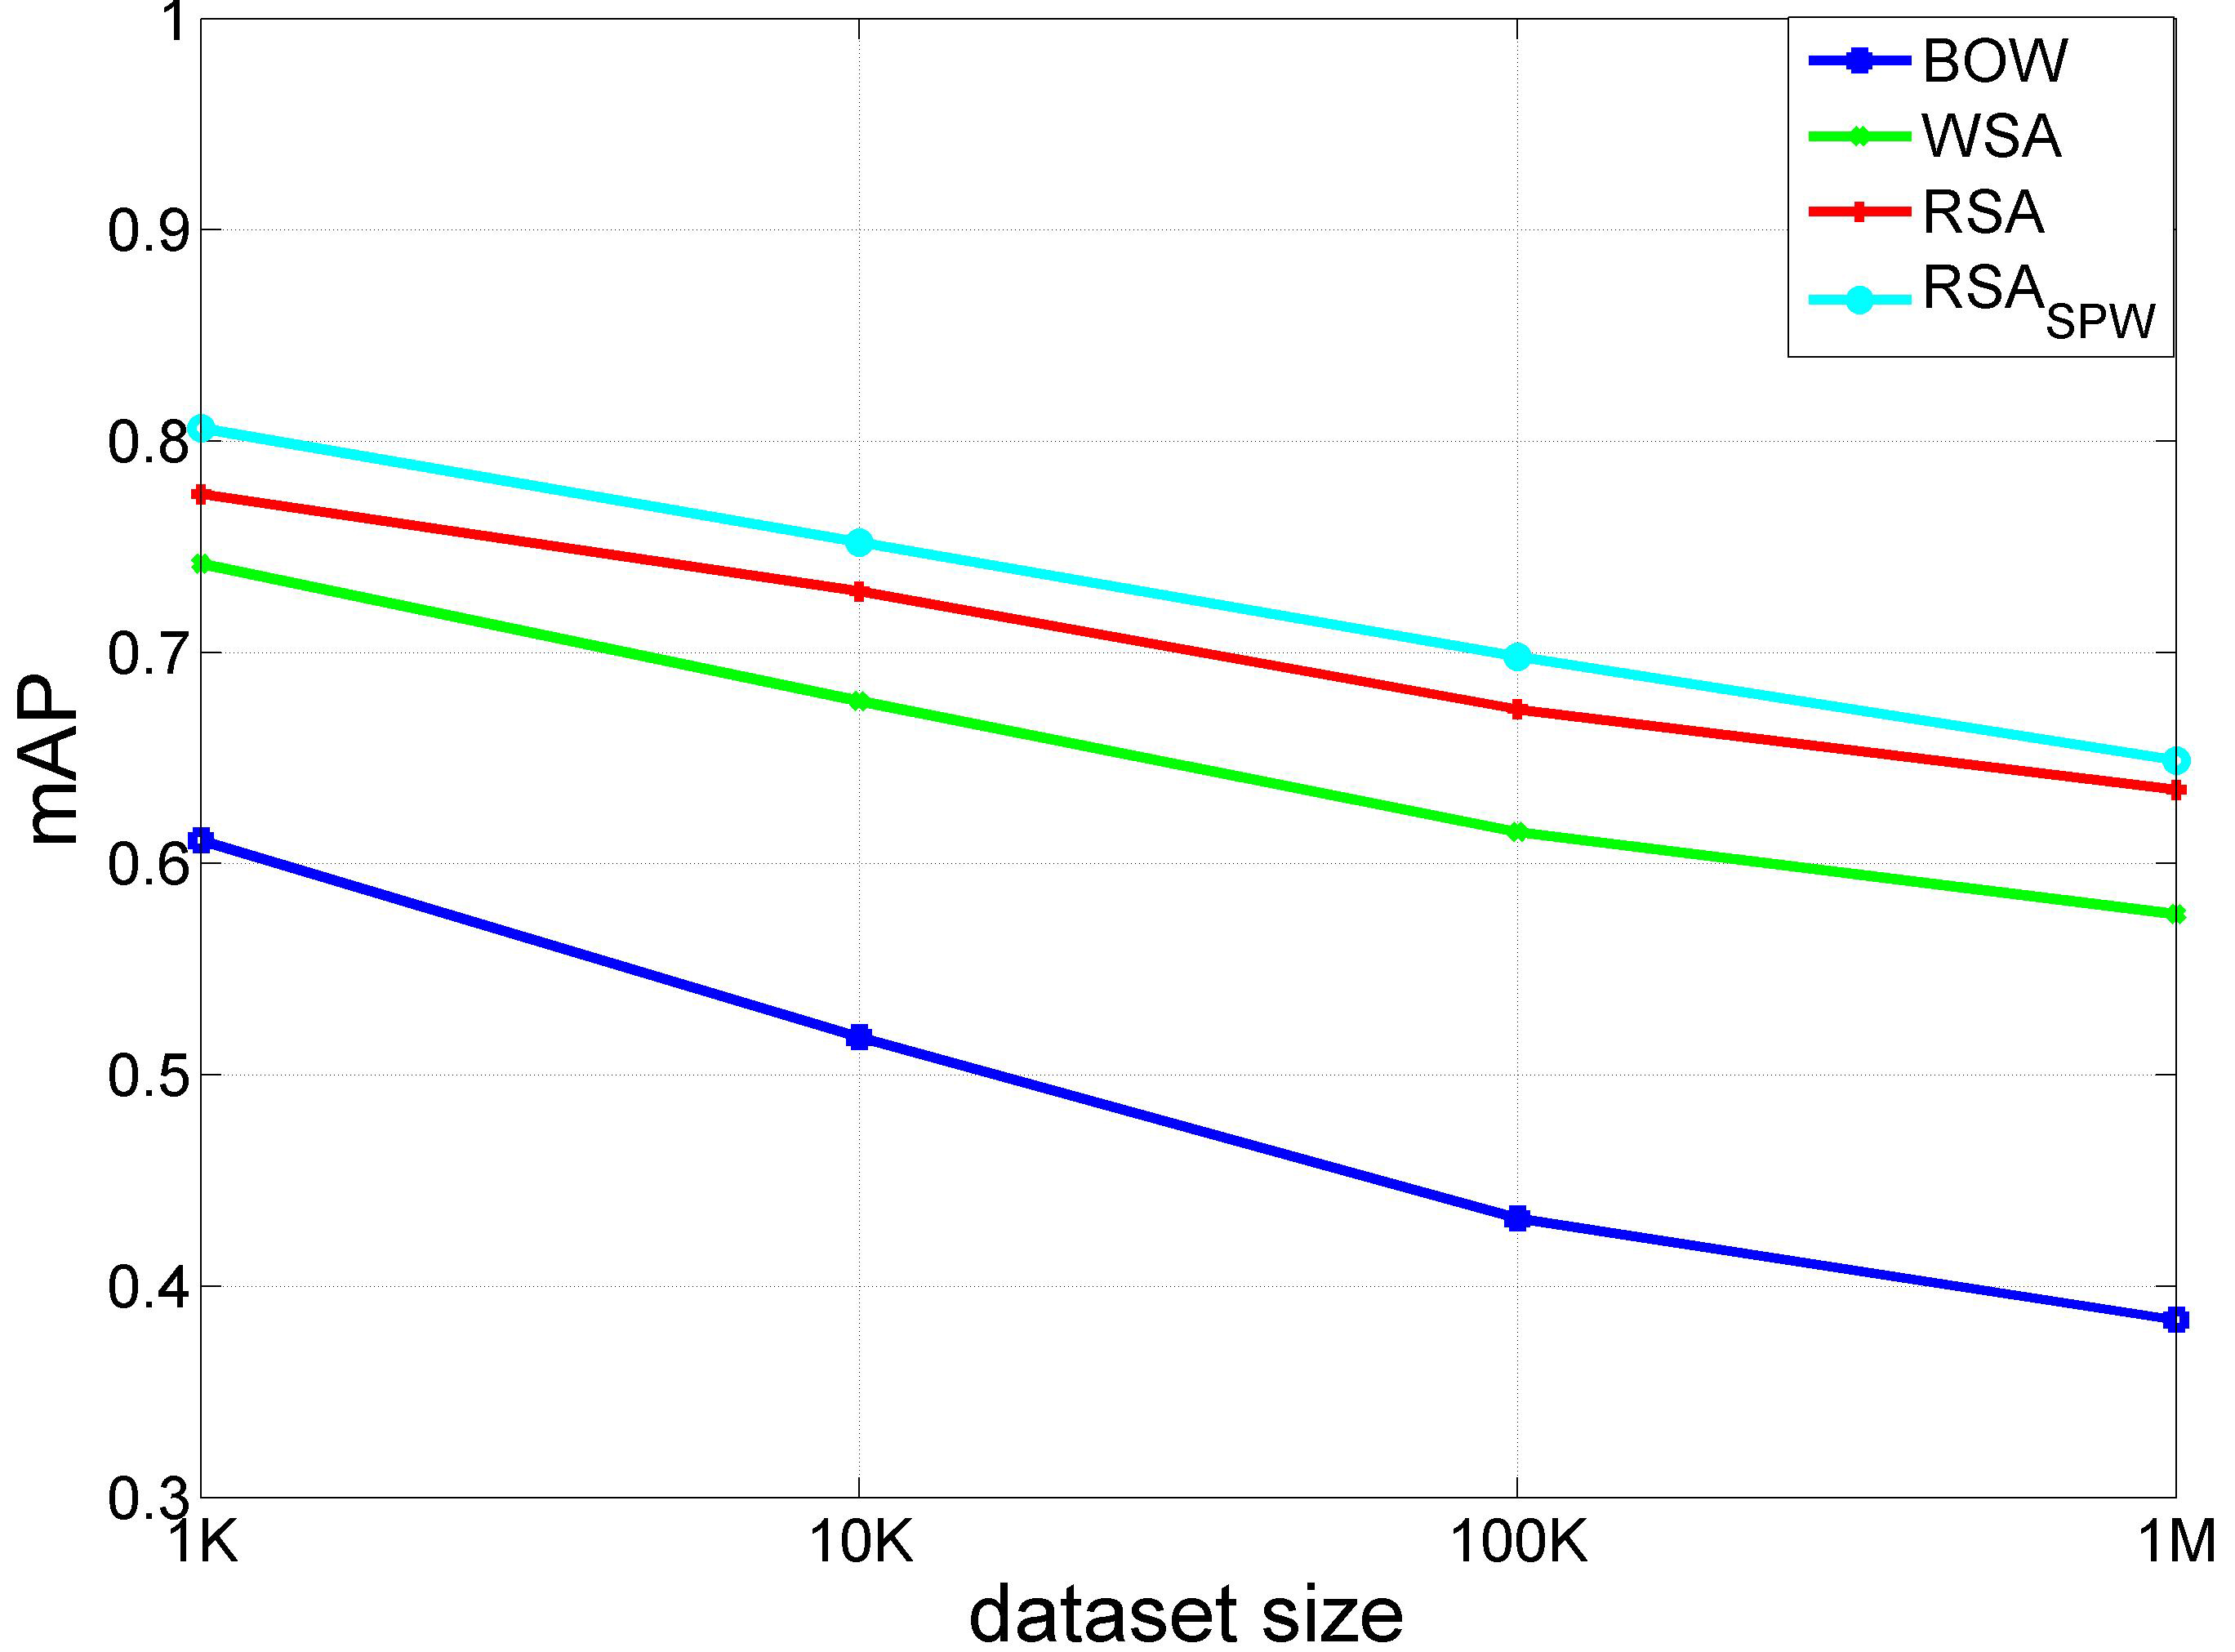
\includegraphics[width=0.6\textwidth]{large_scale.jpg}
	\caption{在Holidays+Flickr1M数据集上的检索结果}\label{fig:ls}
\end{figure}
为了验证RSA的可扩展性,我们在Holidays+Flickr1M数据集上进行了实验(数据集图片总量超过一百万)。图\ref{fig:ls}描绘了RSA、WSA和BoW baseline在大规模数据集下的检索性能,其中字典大小为200K。通过图\ref{fig:ls}我们可以看出在图像库达到百万级别时,RSA可以将mAP从0.384提高到0.694,并且RSA的检索结果要比WSA高13\%。另一方面,通过表\ref{tab:time},RSA几何校验算法所带来的时间增加几乎可以忽略不计。这些实验结果表明,RSA不仅可以显著提升BoW检索的准确率,同时不会带来额外的计算复杂度,是大规模图像检索场景下合适的解决方案。

\subsection{对尺度和角度变化的鲁棒性}
由于RSA算法建立在图像特征区域的属性上,一个明显的问题是RSA可不可以解决图片尺度变化和旋转的问题。angle和scale变化的问题是几何校验中的难点,至今没有很好的解决方案。WGC\cite{jegou2008hamming}为了应对上述问题,认为图片只有4个可能的角度并且图片的尺度是不会改变的,这严重限制了该算法的应用场景。由于RSA编码的是图片全局的几何信息,并且具有较强的鲁棒性,所以RSA可以很好的应对图片尺度变化和旋转的问题。

\subsubsection{图片的尺度变化}
由于图片尺度的变化不会影响点在$S_{Property}$中的相对位置关系,所以RSA不受图片尺度变化的影响。\ref{fig:rsa_s}展示了RSA在Copydays上的检索结果。其中,Copydays上的图片只包含尺度变化,我们使用P@N来度量检索结果,10代表最高准确率。通过图\ref{fig:rsa_s}我们发现,RSA与BoW具有相似的检索结果,这表明RSA不受图片尺度变化的影响,并且SpW同样可以显著提高检索性能。

\subsubsection{图片的旋转}
图片的旋转会改变点在$S_{Property}$的相对位置,但是我们提出的旋转的RSA向量可以很好的应对这个问题。图\ref{fig:rsa_r}展示了旋转的RSA在Holidays数据集上的部分检索结果。其中,绿框表示查询图片,每个查询图片都有旋转版本的相似图片,红框表示没有找到的相似图片。通过图\ref{fig:rsa_r},我们可以看出这些旋转的相似图片几乎可以被RSA算法正确检索。

\begin{figure}[h]
	\centering
	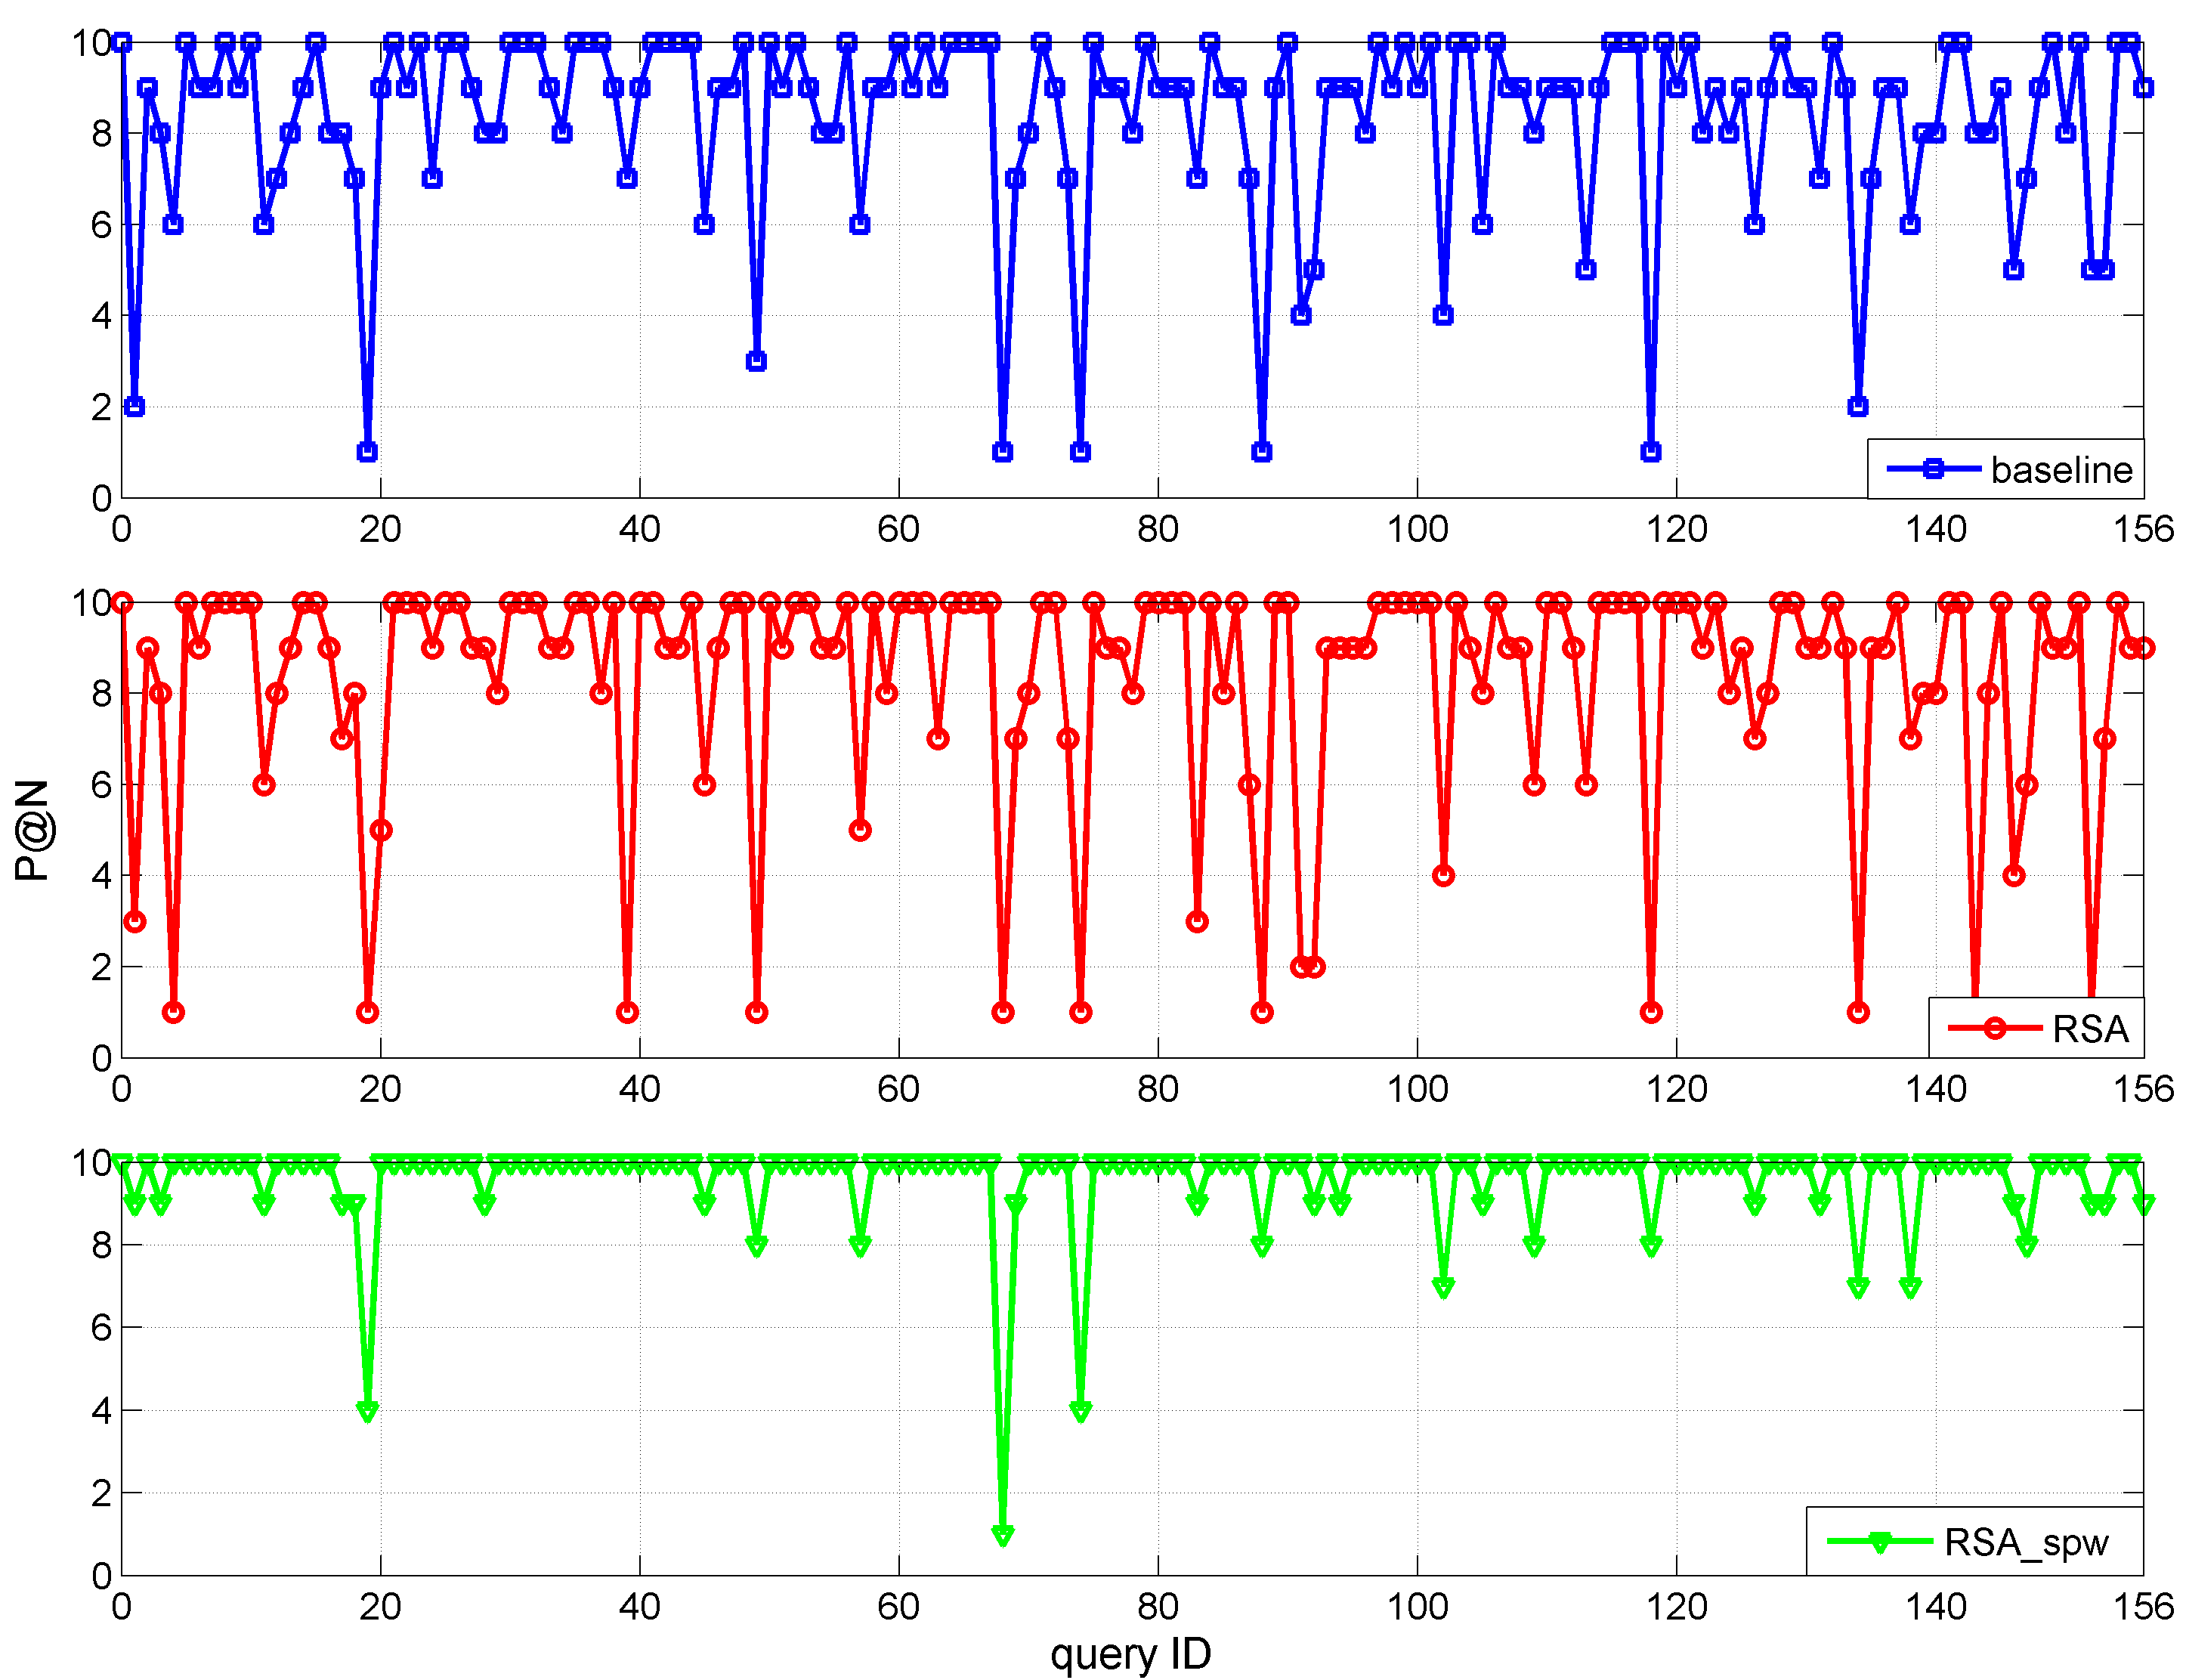
\includegraphics[width=0.8\textwidth]{scale.png}
	\caption{RSA算法在Copydays上的检索结果}\label{fig:rsa_s}
\end{figure}

\begin{figure}[h]
	\centering
	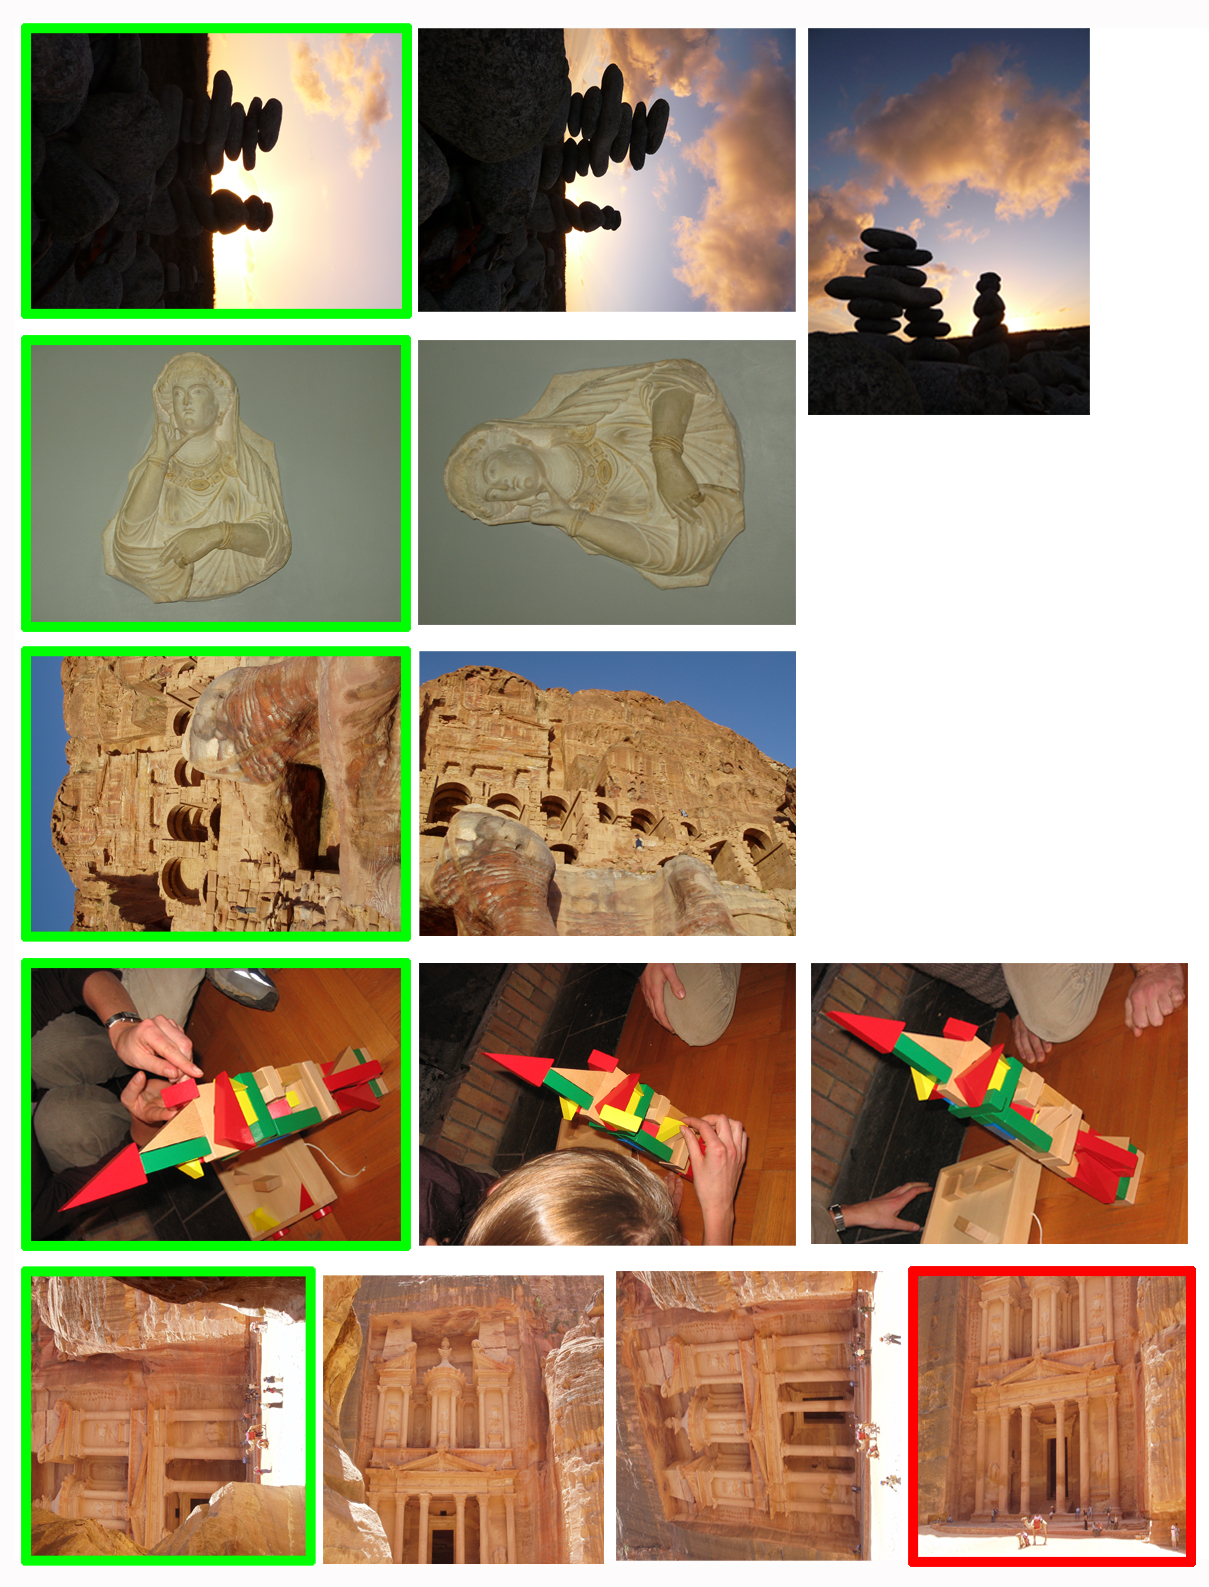
\includegraphics[width=0.8\textwidth]{rotation.jpg}
	\caption{RSA算法在Holidays上的检索结果}\label{fig:rsa_r}
\end{figure}

\section{本章小结}
本章节详细介绍了RSA算法。RSA算法可以明显的提高BoW图像检索的性能。RSA的核心思想是为图片建立Region Property Space(RPS),编码RPS中点的分布特性并在检索时对视觉单词进行几何校验。在RPS中的点具有两点特性:
\begin{enumerate}
	\item 具有明显的分布规律;
	\item 他们几乎不会出现在同一个位置上。
\end{enumerate}
基于第一个特性,我们提出了Spatial Weighting(SpW),SpW显著的提高的RSA的性能,而第二个特性保证了RSA可以对视觉单词进行较强的几何校验。通过量化,RSA在不影响检索效果的情况下占用了更少的内存。我们在三个标准数据集上对RSA算法进行了全面的测试。实验结果表明,RSA算法可以达到与state-of-the-art相近的检索精度。由于不需要后校验和先验知识,对尺度、角度变化不敏感,所以RSA适用于一般的大规模图像检索场景。




